\documentclass{article}
\usepackage[utf8]{inputenc}
\usepackage{capt-of} % Für captionof
\usepackage{hyperref} % Für Links

\title{Macherdaach-Badge-Dockingstation \\ Lötanleitung \\ [1cm]
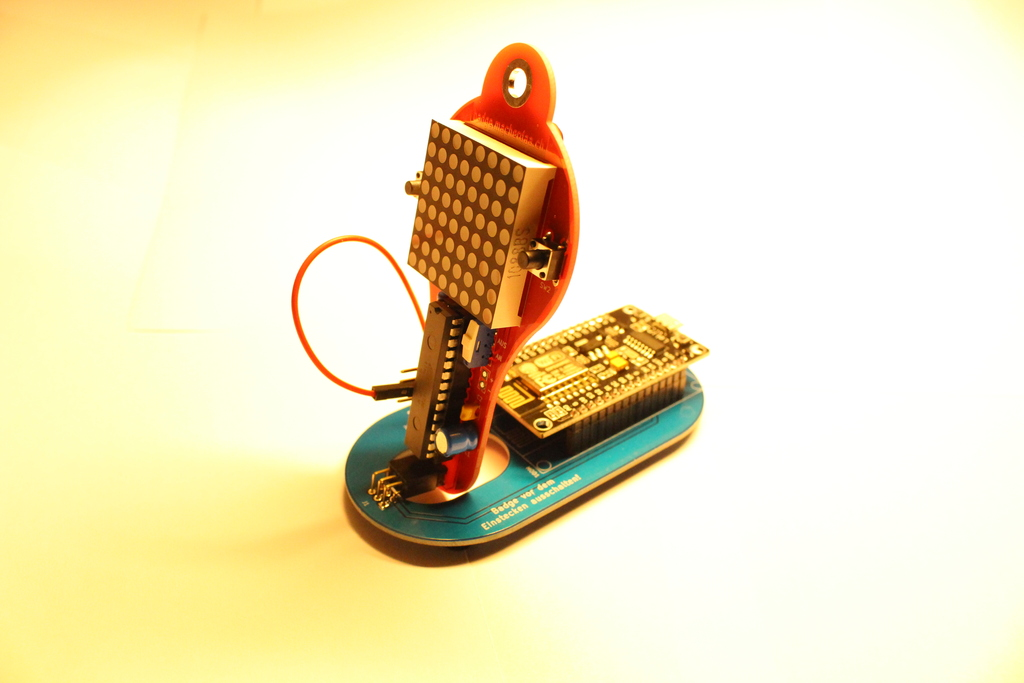
\includegraphics[width=\textwidth]{Bilder2019/IMG_6506.png}
}
\date{September 2019}
\author{casartar\\peter.scheydt@ztl.space}

\usepackage{natbib}
\usepackage{graphicx}
\usepackage[ngerman]{babel} % Macht aus Figure -> Abbildung

\setlength{\parindent}{0pt} % Keine Einrückung nach Absatz

\usepackage{geometry} % Seitenränder ein bisschen schmaler
\geometry{
  left=2cm,
  right=2cm,
  top=2cm,
  bottom=2cm,
  bindingoffset=5mm
}

\begin{document}

\maketitle
\newpage
\section{Einleitung}

Das Macherdaach-Badge-Dock ist für all jene gedacht, die schon ein Macherdaach-Badge haben und noch etwas anderes löten wollen. Mit diesem kleinen Bausatz bieten wir die die Möglichkeit, dein Macherdaach-Badge, egal ob das gelbe vom letzten Jahr (mit einem kleinen Firmware-Update) oder das rote von diesem Jahr, mit dem Internet zu verbinden. Lass dich überraschen, wie es funktioniert...

\section{Die Bauteile stellen sich vor}
Alle Bauteile, die du für deine Dock brauchst, findest du in einer Tüte. Du bekommst sie von einem der freundlichen Helfer am Tisch überreicht.

Folgende Bauteile sollten in der Tüte drin sein:

\begin{enumerate}
	\item Macherdaach-Badge-Dock-Platine
	\item einreihige Stiftleiste 4 Pins
	\item zweireihige Buchsenleiste 3 Pins gewinkelt
	\item zwei einreihige Buchsenleisten 15 Pins
	\item drei Gummifüße
	\item Jumperkabel
	\item LoLin NodeMcu V3
\end{enumerate}



\begin{center}
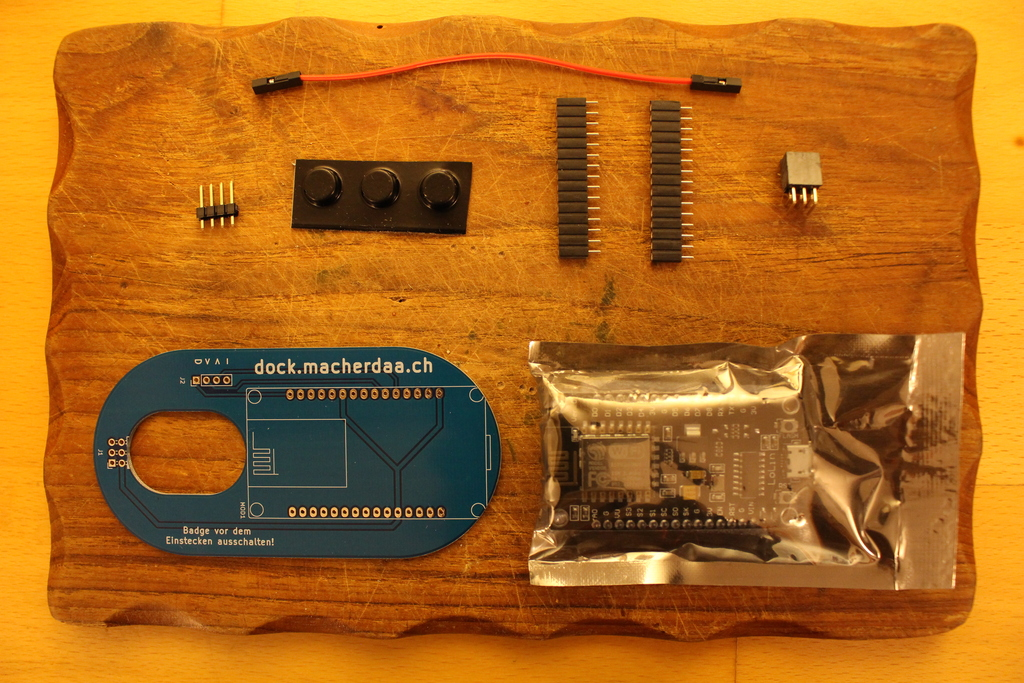
\includegraphics[width=\textwidth]{Bilder2019/IMG_6462.JPG}
\captionof{figure}{Alle Bauteile auf einen Blick}
\label{fig:all_components}
\end{center}

\section{Dokumentation ist alles}

Die Hardware, Software und selbstverständlich diese Anleitung, sind Open Source. Wenn du sie dir ansehen, sie herunterladen oder daran mitarbeiten möchtest, musst du nur folgenden Links folgen:

\begin{itemize}
	\item \url{https://github.com/casartar/MacherDaachBadgeDockFirmware} oder \url{https://dock.macherdaa.ch}
	\item \url{https://github.com/casartar/MacherDaachBadgeDockHardware}
	\item \url{https://github.com/casartar/MacherDaachBadgeDockDoku}
\end{itemize}

Oder suche auf github.com nach Macherdaach.

\section{Jetzt geht es richtig los}
Als allererstes musst du den LoLin NodeMcu auspacken. Am besten benutzt du die Zange, um die Plastikverpackung zu öffnen.

\vspace{1cm}

\begin{minipage}[b]{0.5\textwidth}
	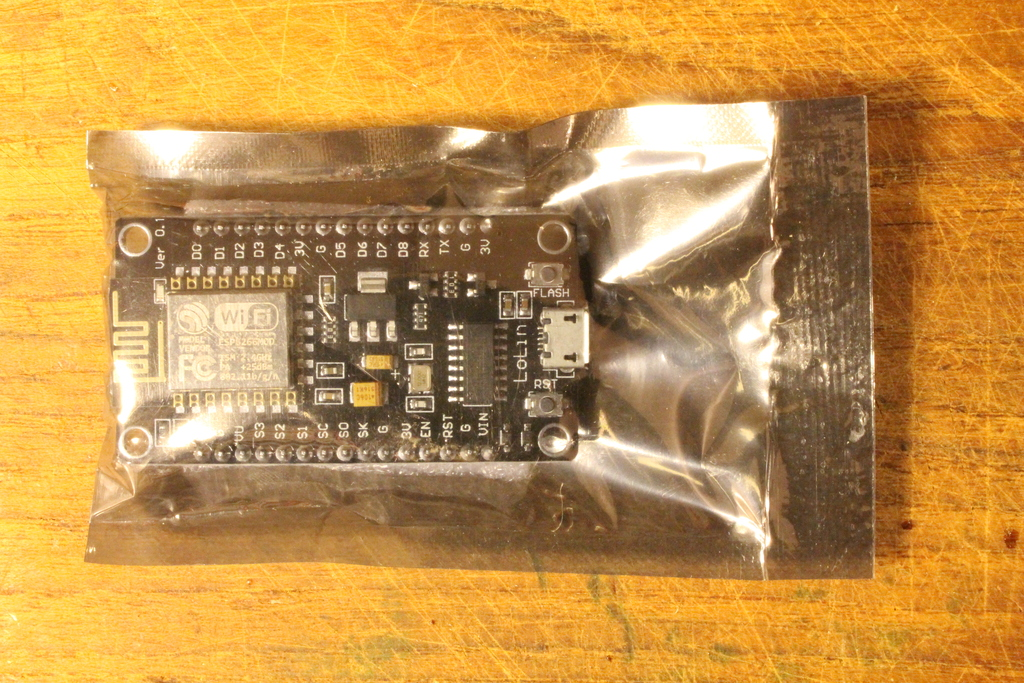
\includegraphics[width=\textwidth]{Bilder2019/IMG_6451.JPG}
	%\captionof{figure}{}
	%\label{fig:}
\end{minipage}
\begin{minipage}[b]{0.5\textwidth}
	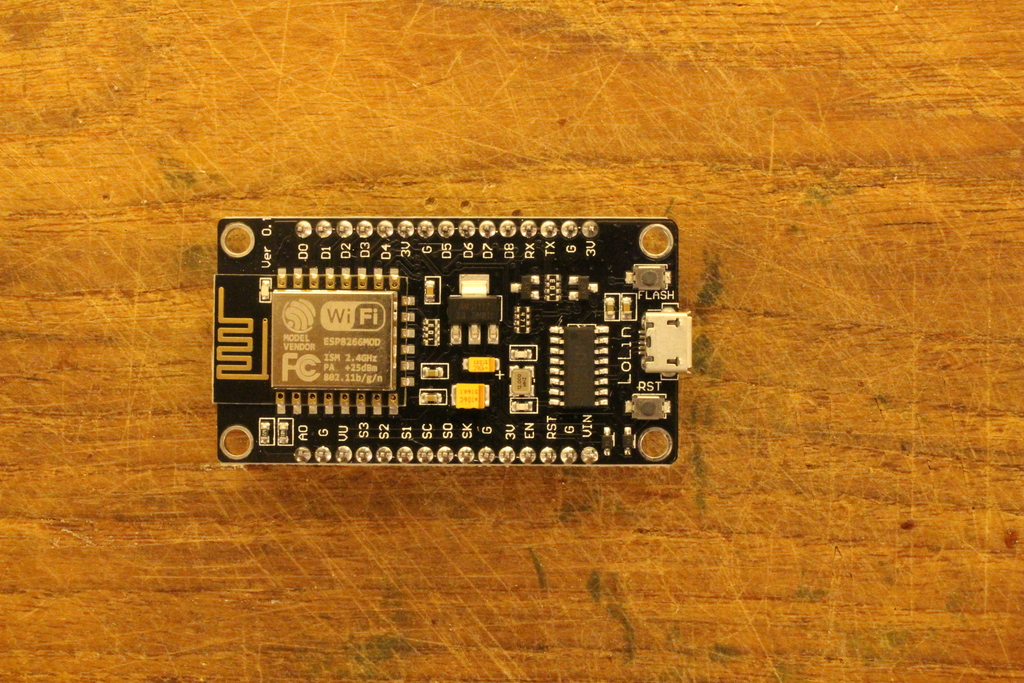
\includegraphics[width=\textwidth]{Bilder2019/IMG_6452.JPG}
	%\captionof{figure}{}
	%\label{fig:}
\end{minipage}

\subsection{Zwei einreihige Buchsenleisten 15 Pins - MOD1}
Die beiden Buchsenleisten musst du auf die Stiftleisten des LoLin NodeMcu stecken. Die Anzahl der Pins stimmt genau überein, es kann also nichts schief gehen. Es kann aber sein, dass die Stiftleisten ein bisschen verbogen sind. Dann musst du ein bisschen rumtüfteln, um die Buchsenleisten richtig aufgesteckt zu bekommen.

\vspace{1cm}

\begin{minipage}[b]{0.5\textwidth}
	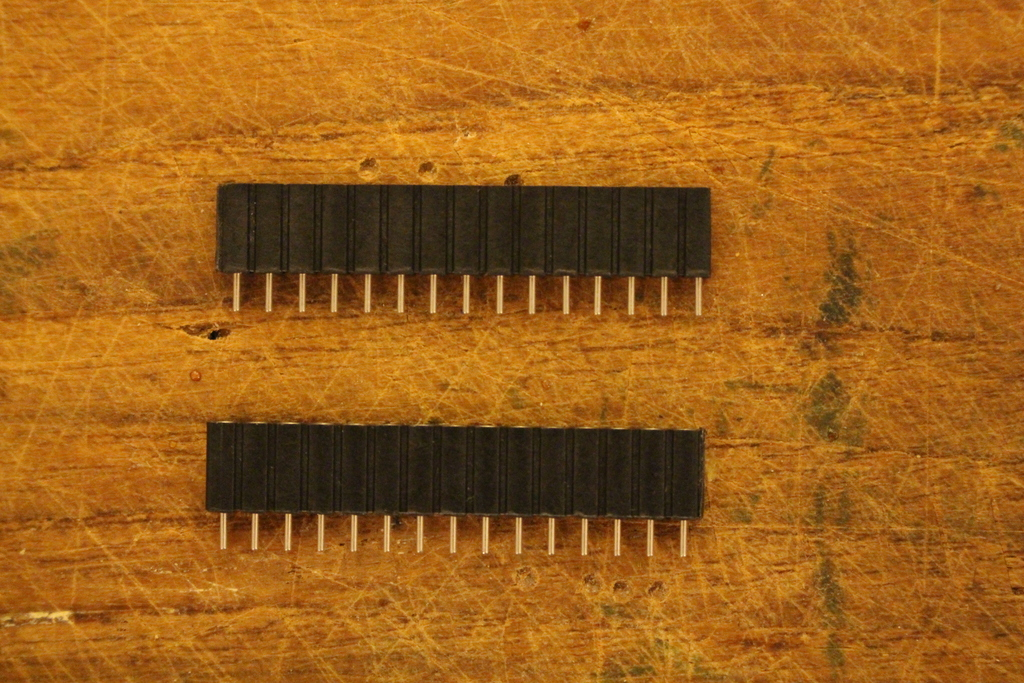
\includegraphics[width=\textwidth]{Bilder2019/IMG_6454.JPG}
	%\captionof{figure}{}
	%\label{fig:}
\end{minipage}
\begin{minipage}[b]{0.5\textwidth}
	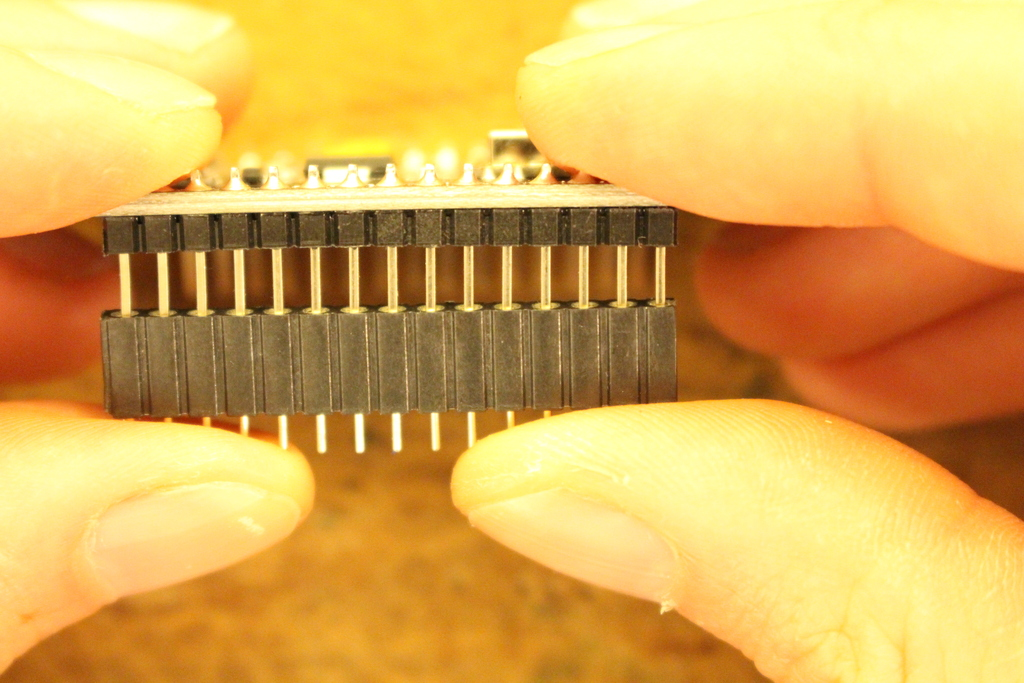
\includegraphics[width=\textwidth]{Bilder2019/IMG_6455.JPG}
	%\captionof{figure}{}
	%\label{fig:}
\end{minipage}

\vspace{0.5cm}

\begin{minipage}[b]{0.5\textwidth}
	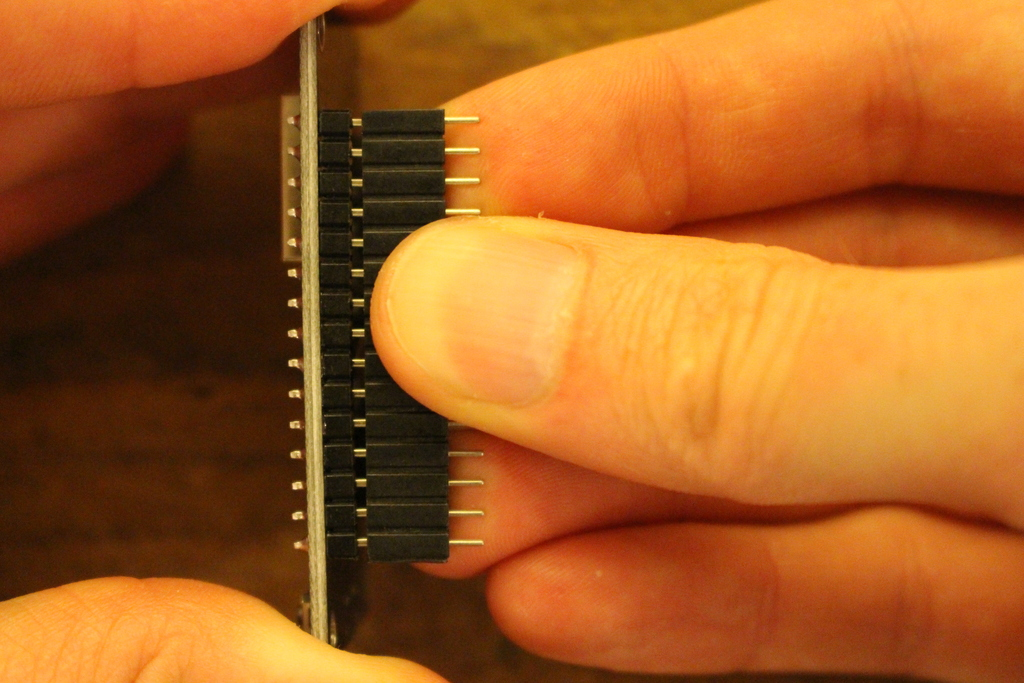
\includegraphics[width=\textwidth]{Bilder2019/IMG_6456.JPG}
	%\captionof{figure}{}
	%\label{fig:}
\end{minipage}
\begin{minipage}[b]{0.5\textwidth}
	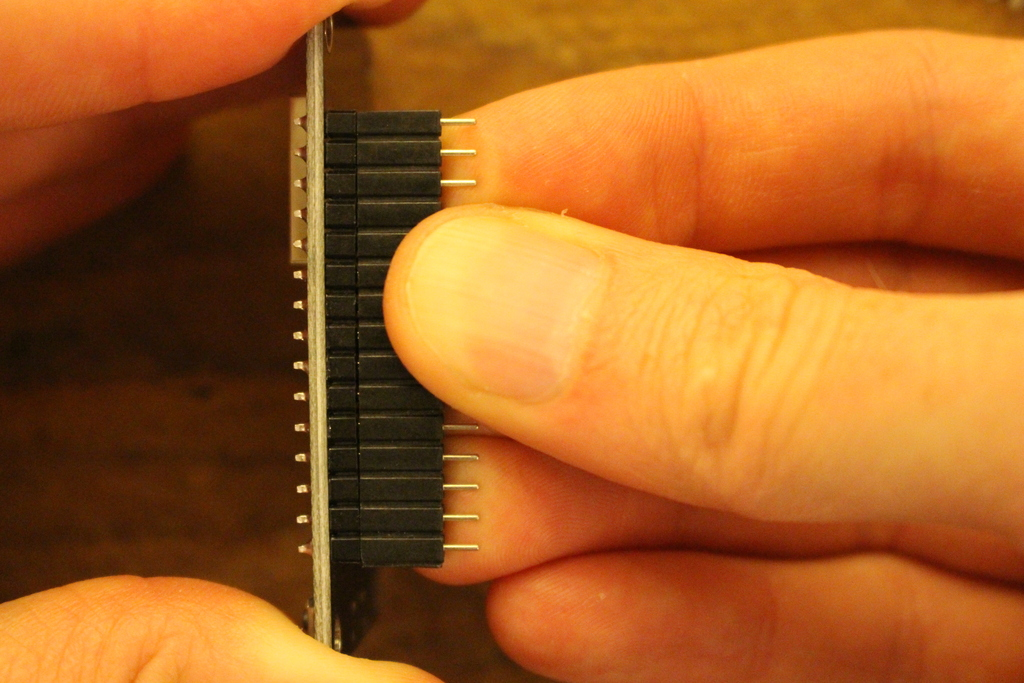
\includegraphics[width=\textwidth]{Bilder2019/IMG_6457.JPG}
	%\captionof{figure}{}
	%\label{fig:}
\end{minipage}

\vspace{0.5cm}

\begin{minipage}[b]{0.5\textwidth}
	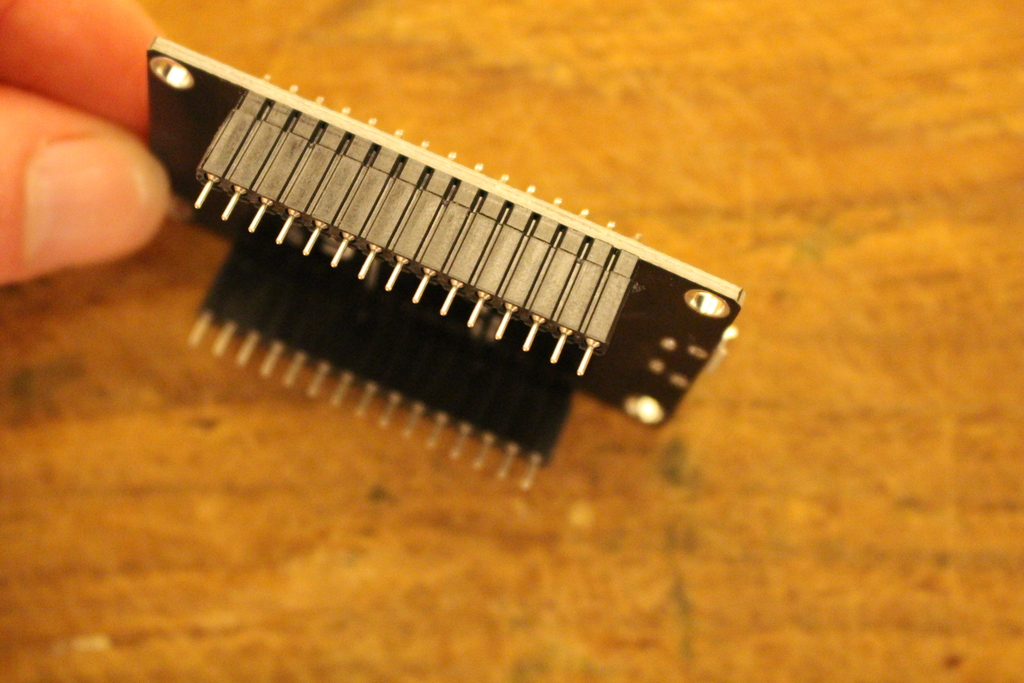
\includegraphics[width=\textwidth]{Bilder2019/IMG_6458.JPG}
	%\captionof{figure}{}
	%\label{fig:}
\end{minipage}

\vspace{0.5cm}

Stecke beide Buchsenleisten auf den LoLin NodeMcu. Anschließend wird das Ganze auf die Platine gesteckt. Bei der Richtung kannst du dich an der meanderförmigen WLAN-Antenne orientieren, die sowohl auf dem LoLin NodeMcu als auch aufgedruckt auf der Platine des Docks zu sehen ist.\\

Nun musst du die Buchsenleisten nur noch mit der Platine verlöten.

\vspace{1cm}

\begin{minipage}[b]{0.5\textwidth}
	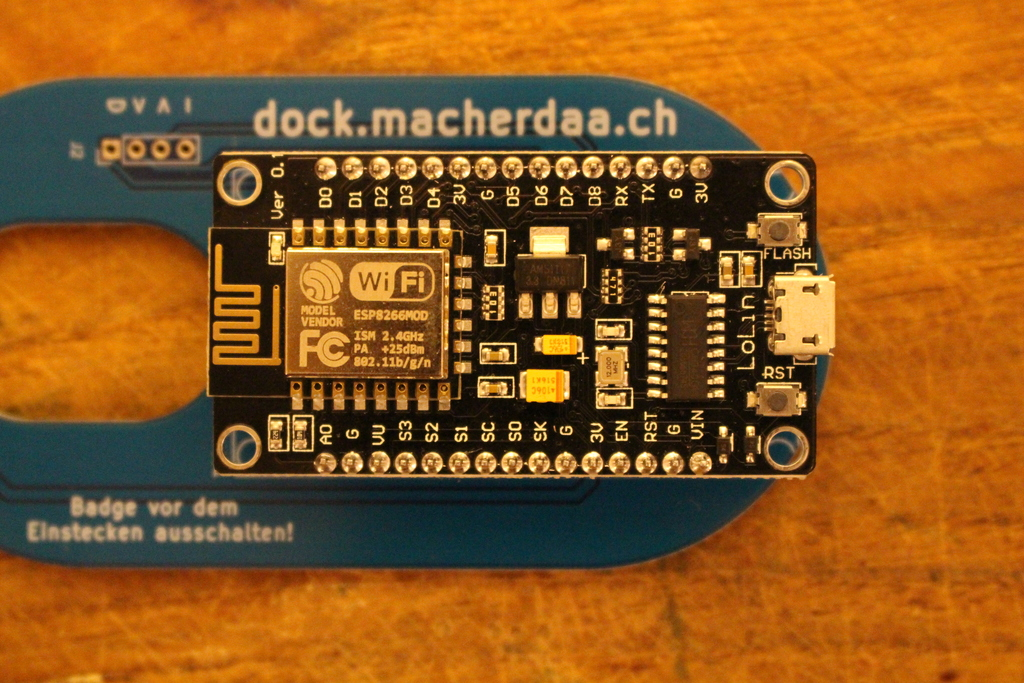
\includegraphics[width=\textwidth]{Bilder2019/IMG_6460.JPG}
	%\captionof{figure}{}
	%\label{fig:}
\end{minipage}
\begin{minipage}[b]{0.5\textwidth}
	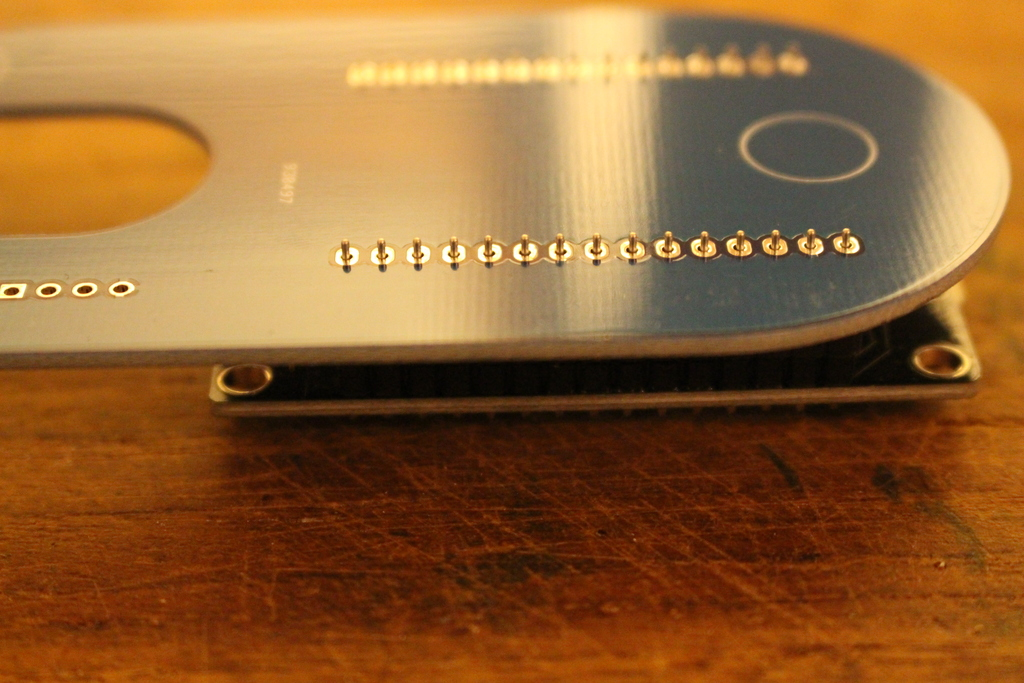
\includegraphics[width=\textwidth]{Bilder2019/IMG_6461.JPG}
	%\captionof{figure}{}
	%\label{fig:}
\end{minipage}

\vspace{0.5cm}

\begin{minipage}[b]{0.5\textwidth}
	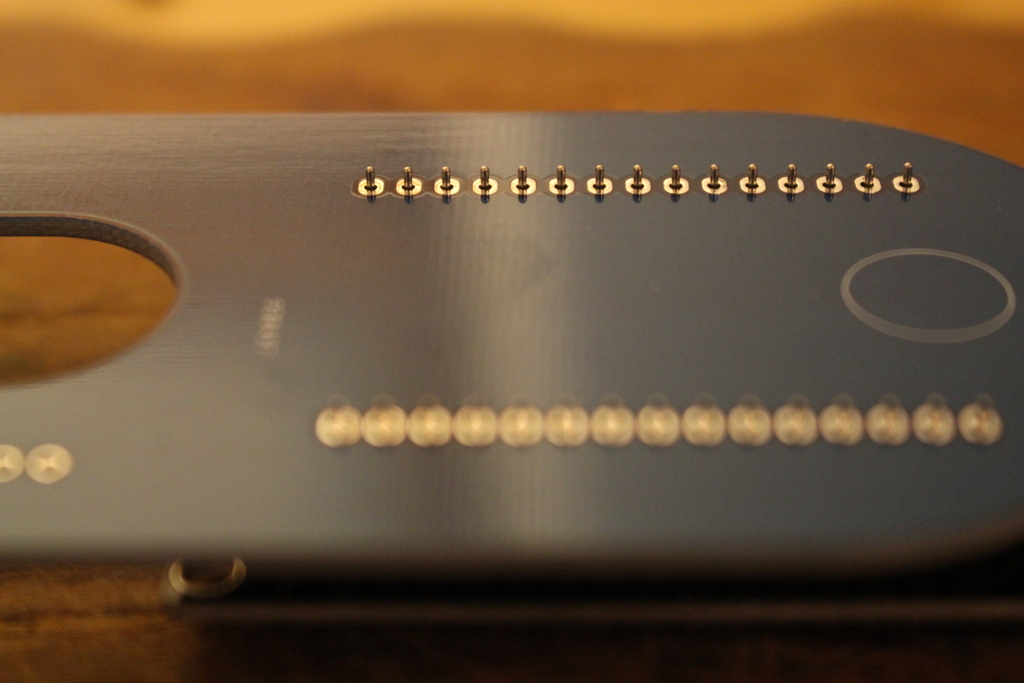
\includegraphics[width=\textwidth]{Bilder2019/IMG_6463.JPG}
	%\captionof{figure}{}
	%\label{fig:}
\end{minipage}
\begin{minipage}[b]{0.5\textwidth}
	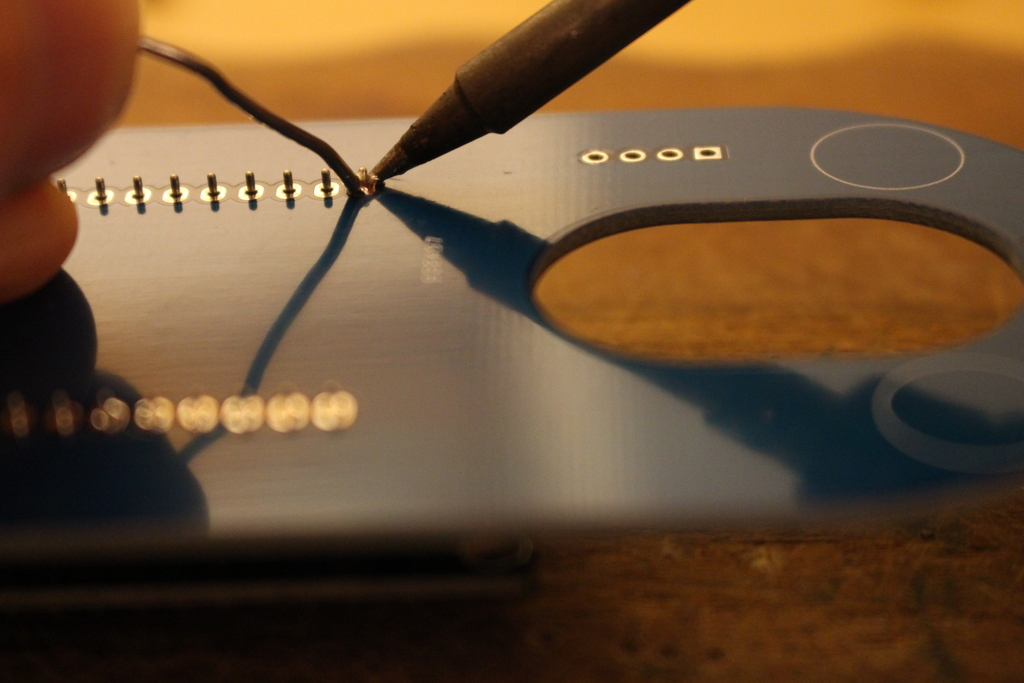
\includegraphics[width=\textwidth]{Bilder2019/IMG_6466.JPG}
	%\captionof{figure}{}
	%\label{fig:}
\end{minipage}

\vspace{0.5cm}

\begin{minipage}[b]{0.5\textwidth}
	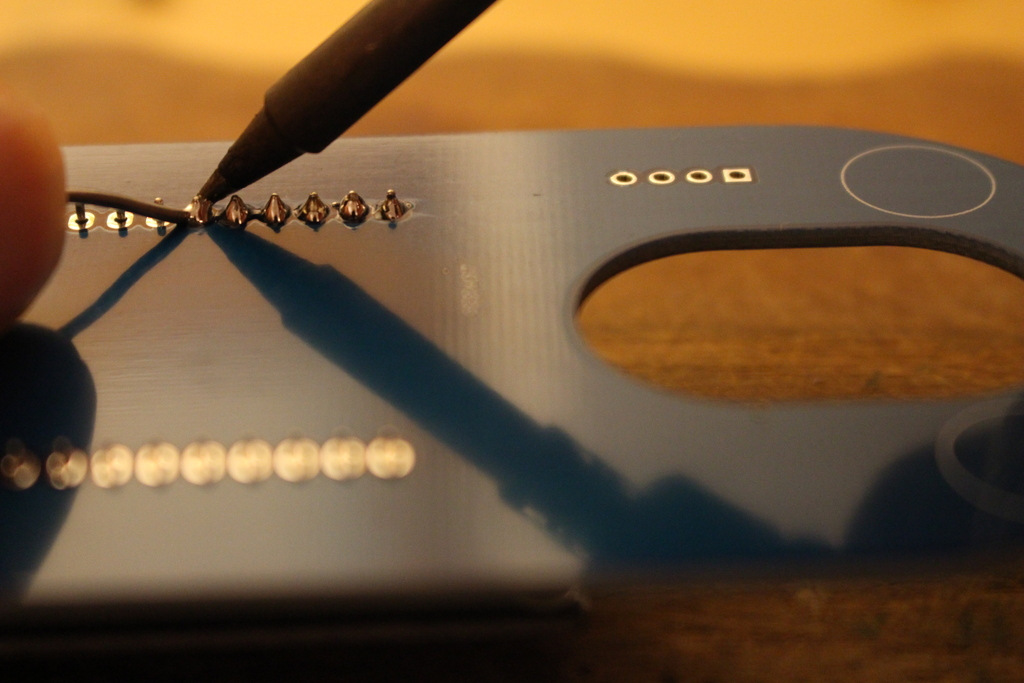
\includegraphics[width=\textwidth]{Bilder2019/IMG_6468.JPG}
	%\captionof{figure}{}
	%\label{fig:}
\end{minipage}
\begin{minipage}[b]{0.5\textwidth}
	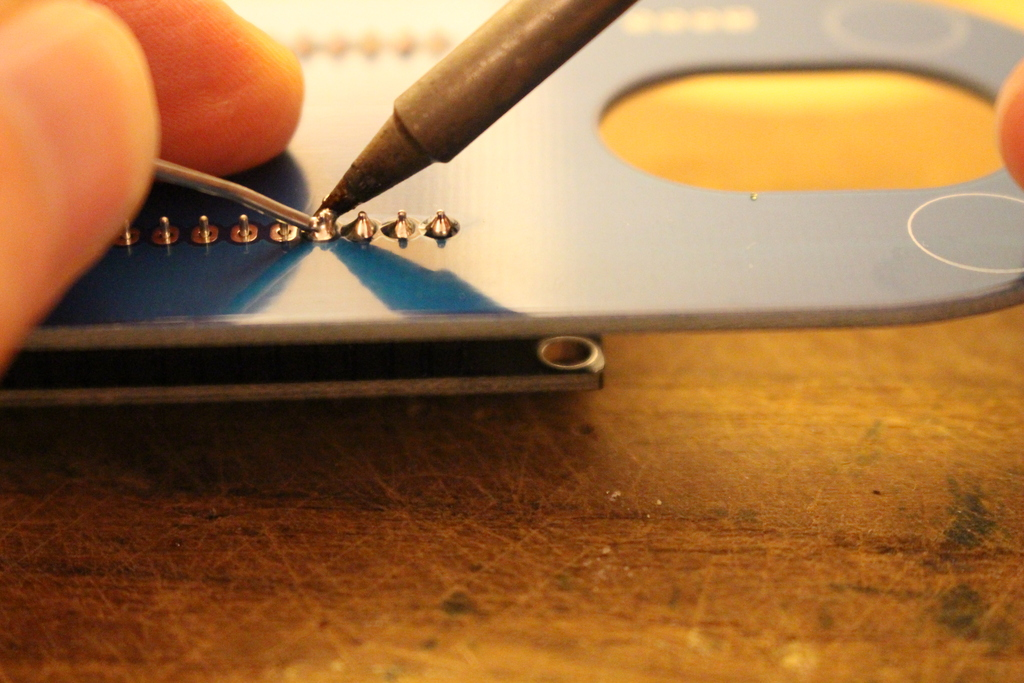
\includegraphics[width=\textwidth]{Bilder2019/IMG_6469.JPG}
	%\captionof{figure}{}
	%\label{fig:}
\end{minipage}

\vspace{0.5cm}

\begin{minipage}[b]{0.5\textwidth}
	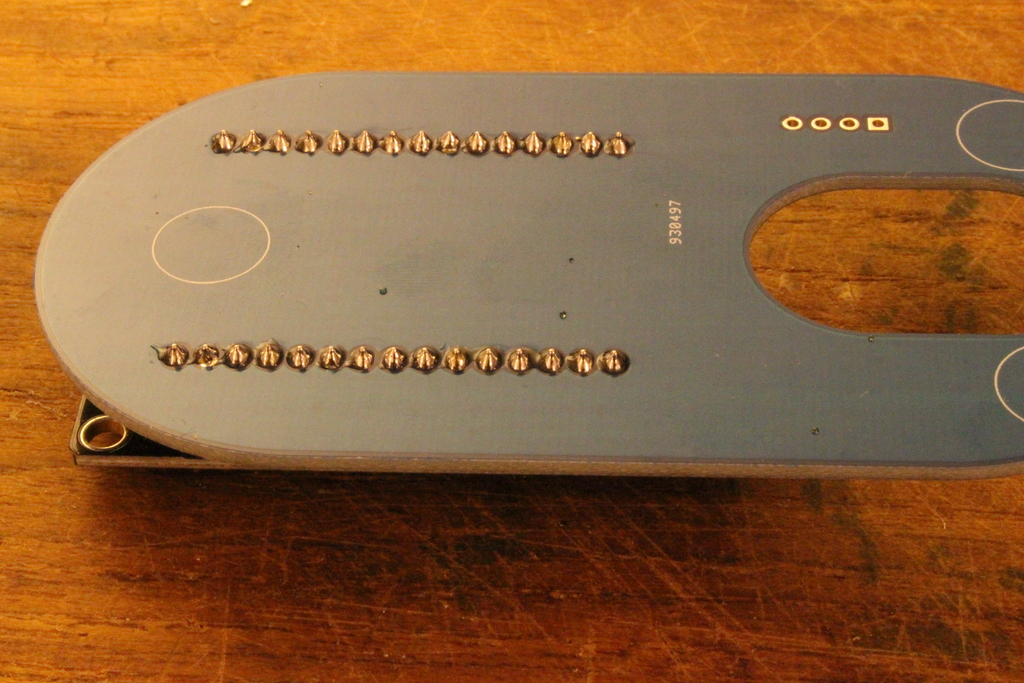
\includegraphics[width=\textwidth]{Bilder2019/IMG_6472.JPG}
	%\captionof{figure}{}
	%\label{fig:}
\end{minipage}

\subsection{Einreihige Stiftleiste 4 Pins - J2}

Als nächstes wird die 4-polige Stiftleiste aufgelötet. Dazu ziehst du am besten den LoLin Nodemcu wieder von den Buchsenleisten ab und legst ihn beiseite.

\vspace{1cm}

\begin{minipage}[b]{0.5\textwidth}
	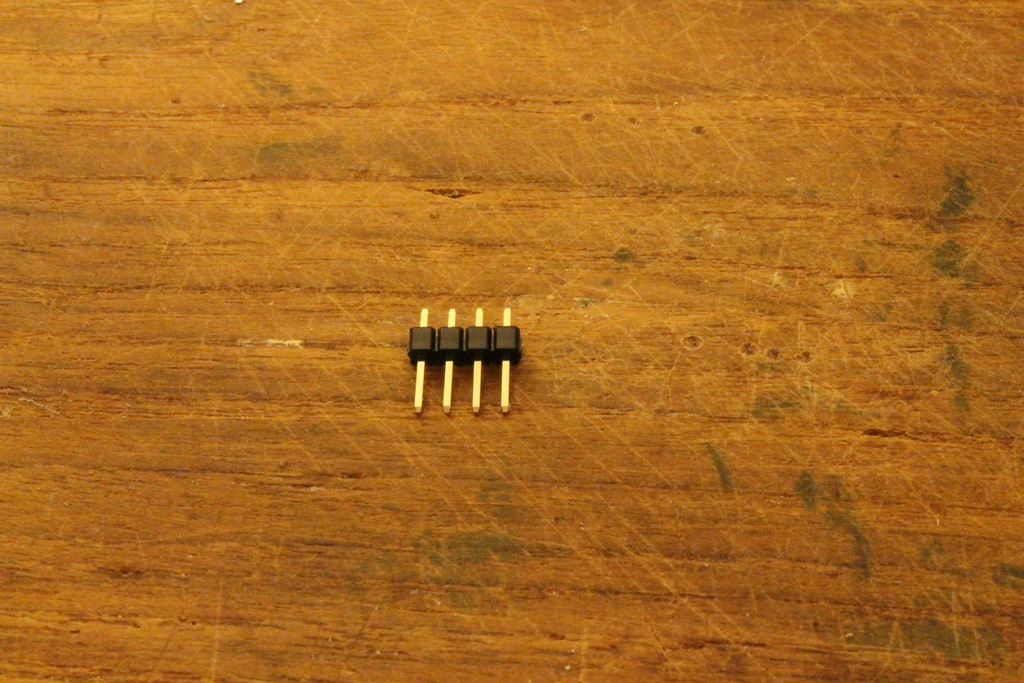
\includegraphics[width=\textwidth]{Bilder2019/IMG_6473.JPG}
	%\captionof{figure}{}
	%\label{fig:}
\end{minipage}
\begin{minipage}[b]{0.5\textwidth}
	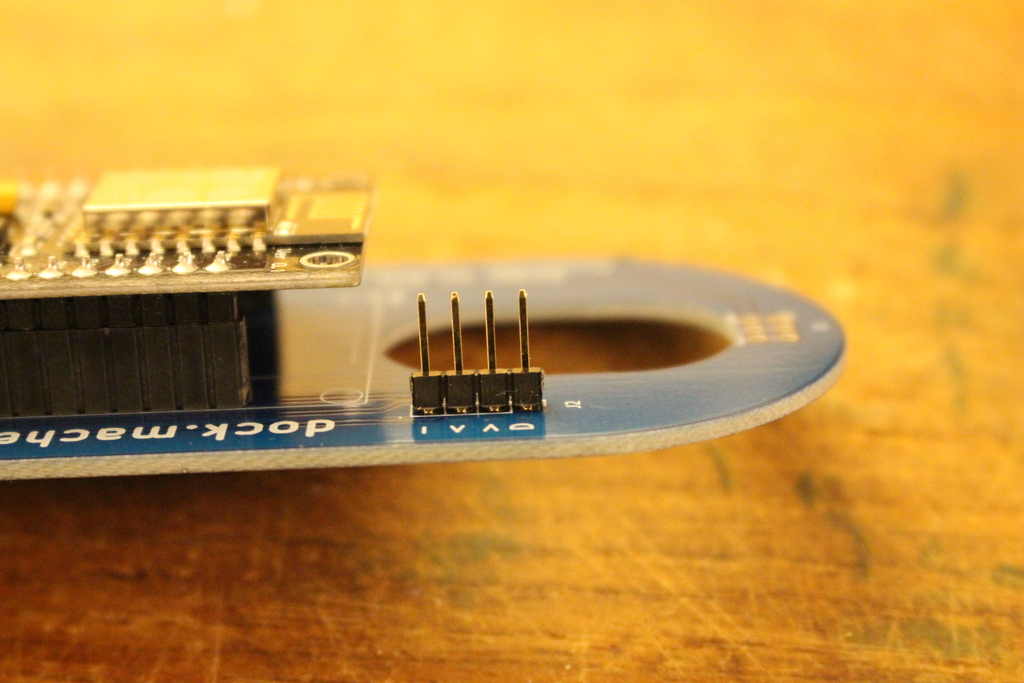
\includegraphics[width=\textwidth]{Bilder2019/IMG_6474.JPG}
	%\captionof{figure}{}
	%\label{fig:}
\end{minipage}

\vspace{0.5cm}

\begin{minipage}[b]{0.5\textwidth}
	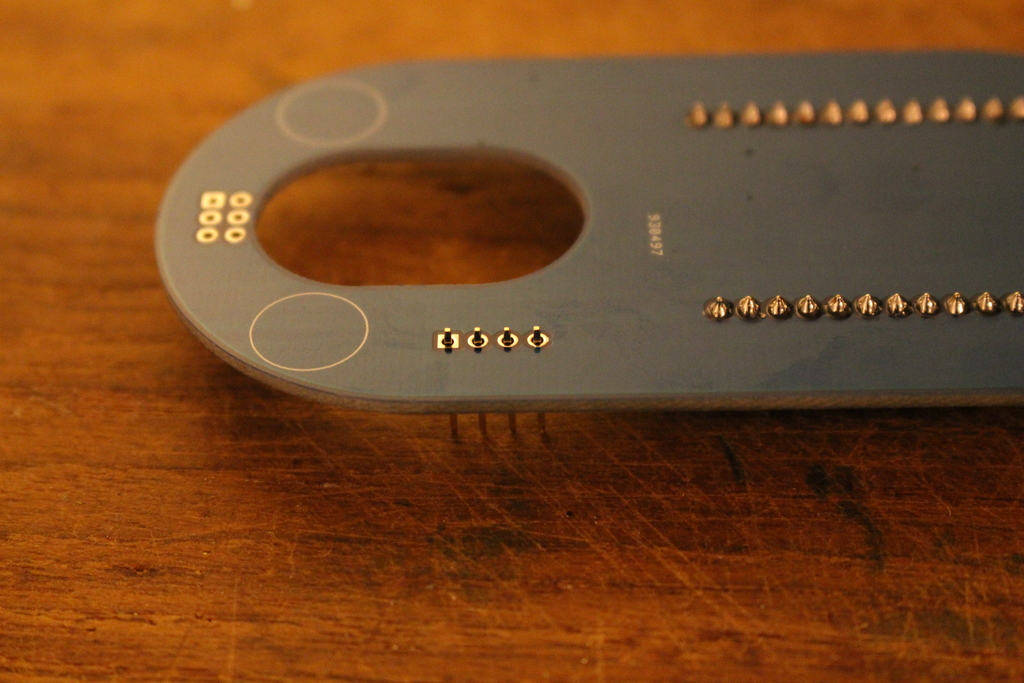
\includegraphics[width=\textwidth]{Bilder2019/IMG_6475.JPG}
	%\captionof{figure}{}
	%\label{fig:}
\end{minipage}
\begin{minipage}[b]{0.5\textwidth}
	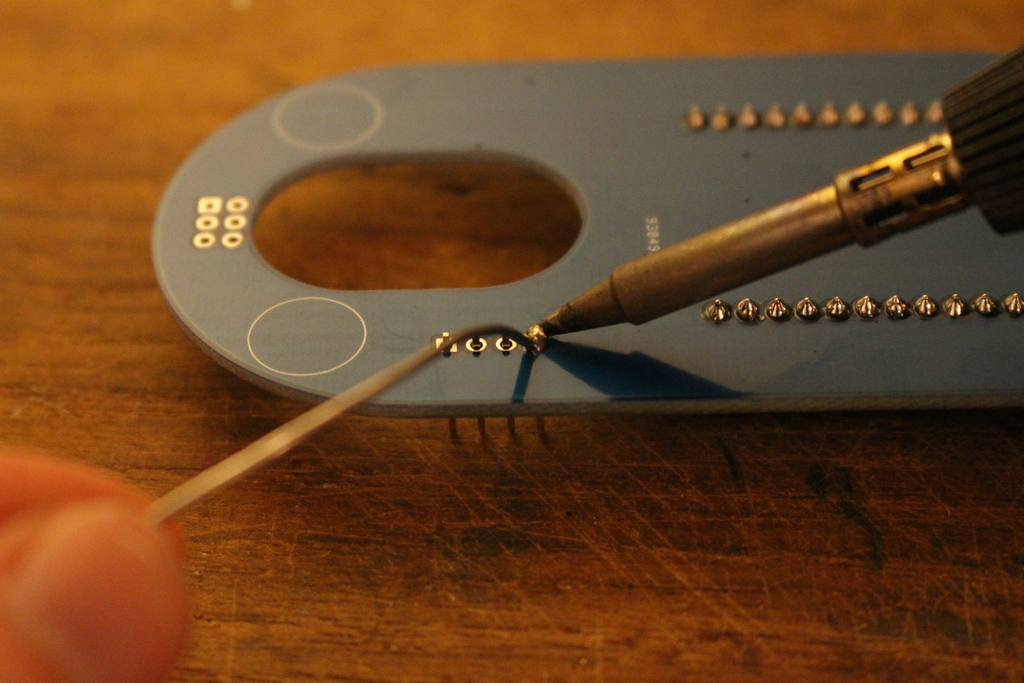
\includegraphics[width=\textwidth]{Bilder2019/IMG_6476.JPG}
	%\captionof{figure}{}
	%\label{fig:}
\end{minipage}

\vspace{0.5cm}

\begin{minipage}[b]{0.5\textwidth}
	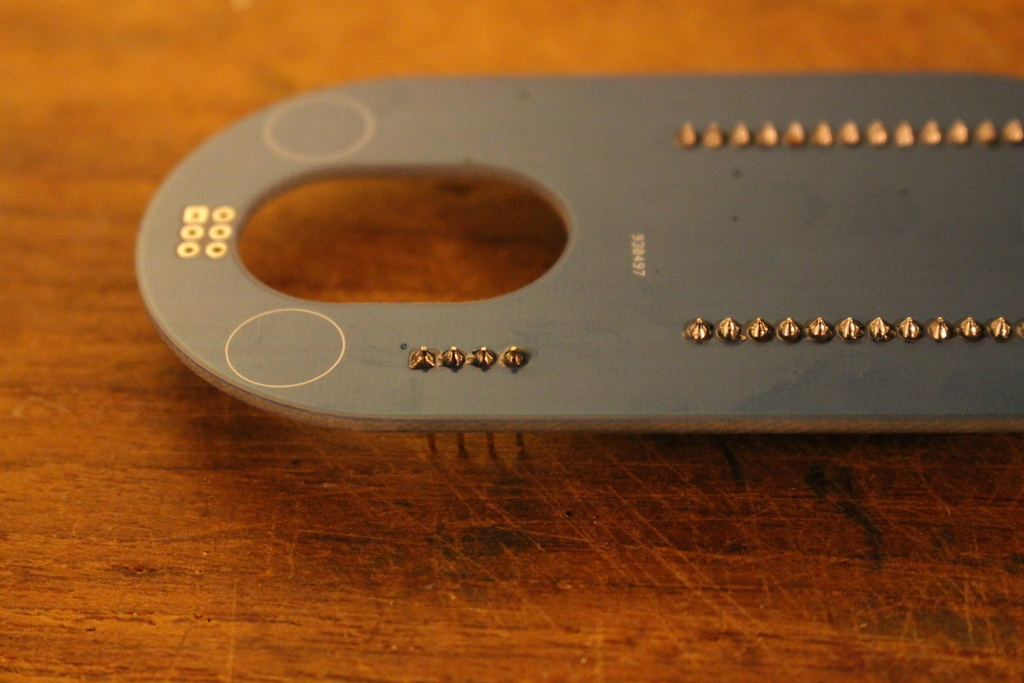
\includegraphics[width=\textwidth]{Bilder2019/IMG_6477.JPG}
	%\captionof{figure}{}
	%\label{fig:}
\end{minipage}

\subsection{Drei Gummifüße}

Die Gummifüße musst du von ihrer Unterlage lösen und dann auf der Unterseite der Dock-Platine auf die weißen Ringe kleben.

\vspace{1cm}

\begin{minipage}[b]{0.5\textwidth}
	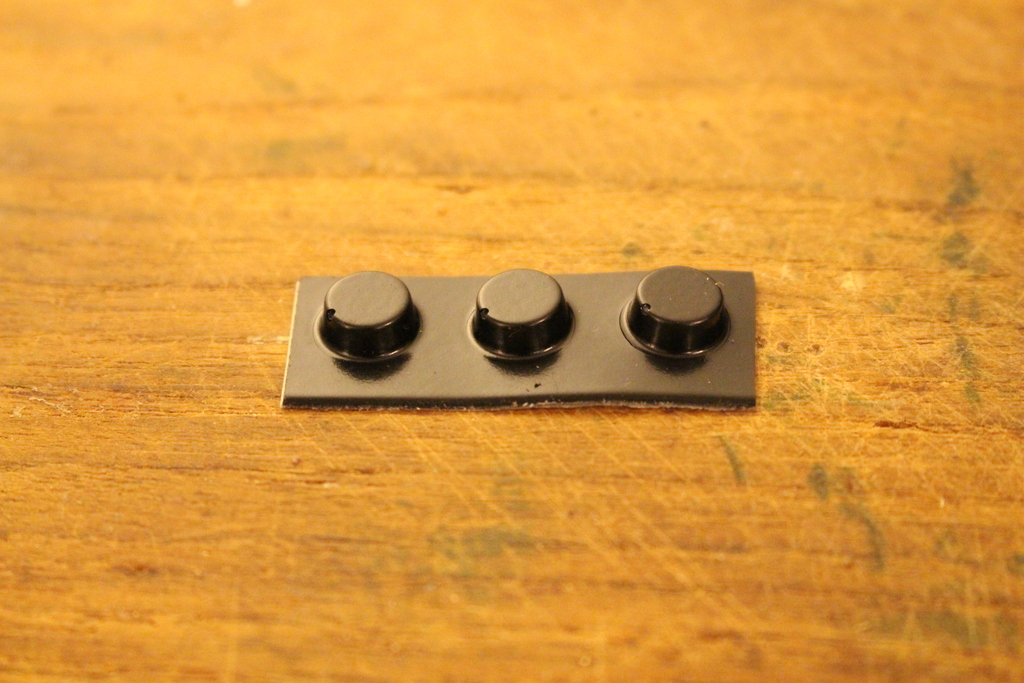
\includegraphics[width=\textwidth]{Bilder2019/IMG_6478.JPG}
	%\captionof{figure}{}
	%\label{fig:}
\end{minipage}
\begin{minipage}[b]{0.5\textwidth}
	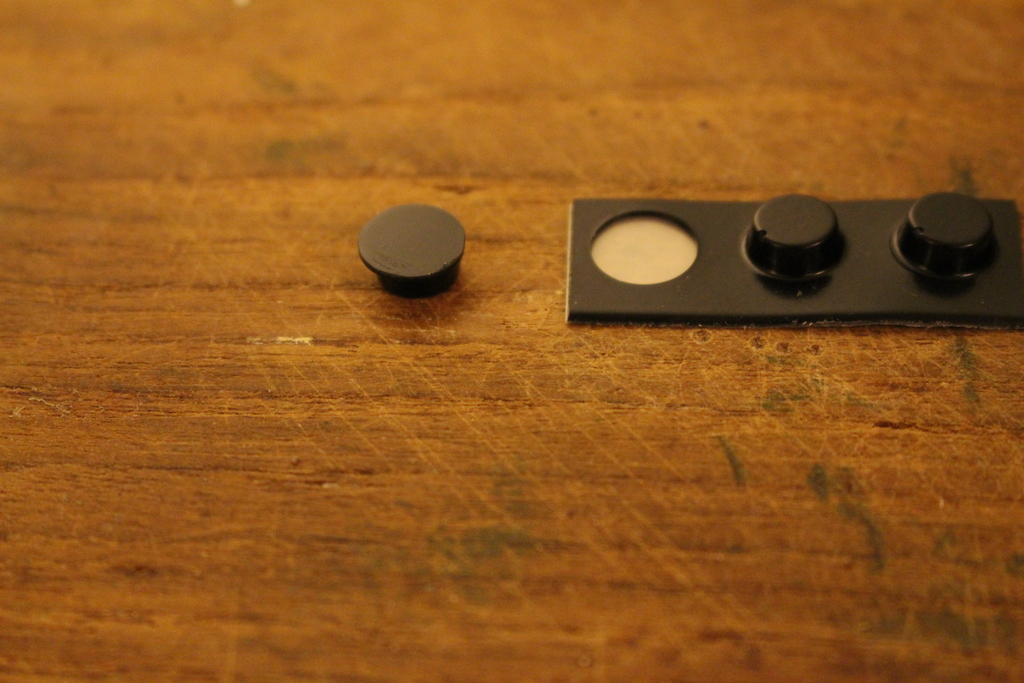
\includegraphics[width=\textwidth]{Bilder2019/IMG_6479.JPG}
	%\captionof{figure}{}
	%\label{fig:}
\end{minipage}

\vspace{0.5cm}

\begin{minipage}[b]{0.5\textwidth}
	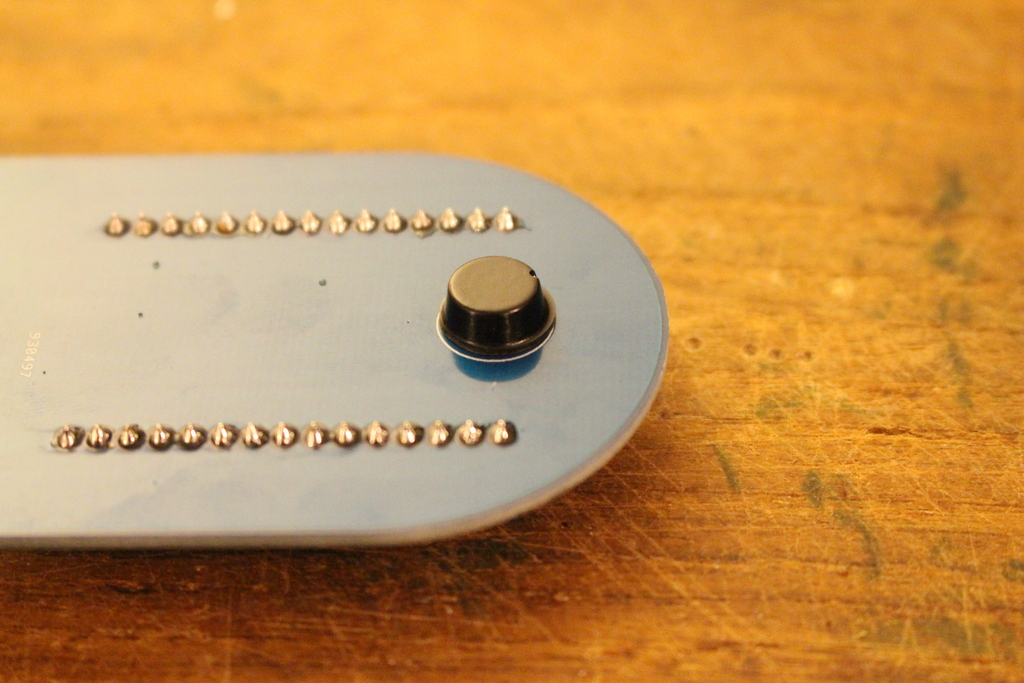
\includegraphics[width=\textwidth]{Bilder2019/IMG_6480.JPG}
	%\captionof{figure}{}
	%\label{fig:}
\end{minipage}
\begin{minipage}[b]{0.5\textwidth}
	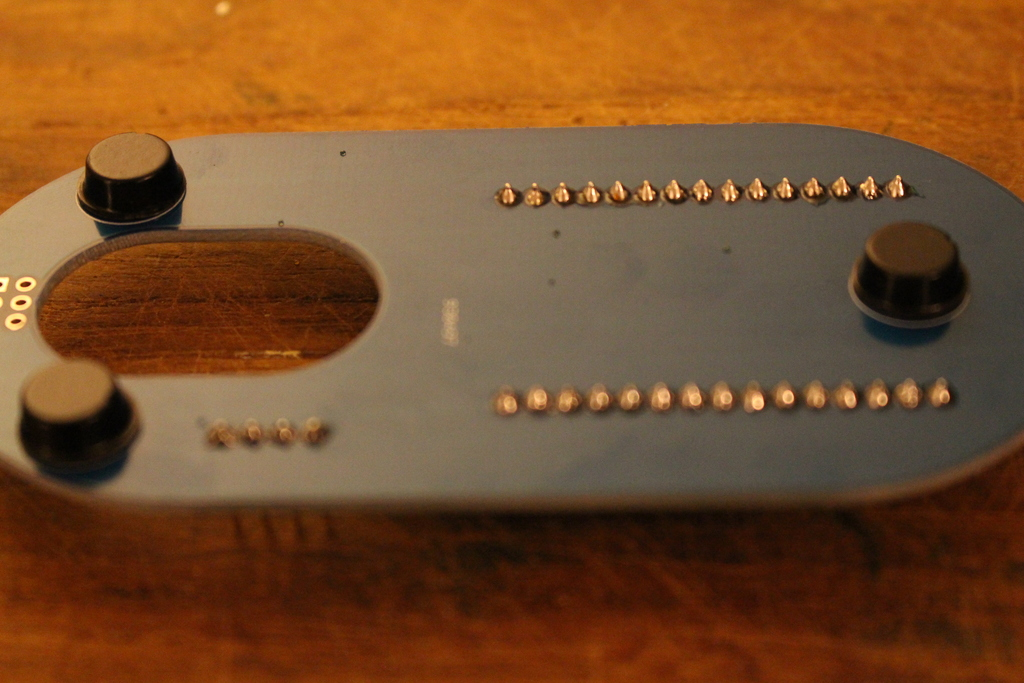
\includegraphics[width=\textwidth]{Bilder2019/IMG_6481.JPG}
	%\captionof{figure}{}
	%\label{fig:}
\end{minipage}

\subsection{Zweireihige Buchsenleiste 3 Pins gewinkelt - J1}

Jetzt kommt der schwierigste Teil, aber keine Angst, so schlimm ist es auch wieder nicht.

Du steckst die doppelreihige, 3-polige Buchsenleiste mit den gewinkelten Pins so auf die 6-polige Stiftleiste am unteren Ende deines Macherdaach-Badges, dass die Pins von der Platine weg zeigen.

Dann steckst du Buchsenleiste samt Macherdaach-Badge auf die Dock-Platine, an der Stelle, die mit J1 gekennzeichnet ist. Justiere das ganze so, dass die Platine des Badges an den Rändern der Aussparung in der Dock-Platine aufliegt. Dabei steht das Badge leicht schräg.

Nun musst du Badge und Dock zur Seite legen und den ersten Pin der Buchsenleiste festlöten. Ist das geschafft, kannst du das Badge abziehen, die Dock-Platine mit der Schrift nach unten hinlegen und die restlichen fünf Pins festlöten.

Als letztes musst du das Macherdaach-Badge und den LoLin NodeMcu wieder aufstecken.

\vspace{1cm}

\begin{minipage}[b]{0.5\textwidth}
	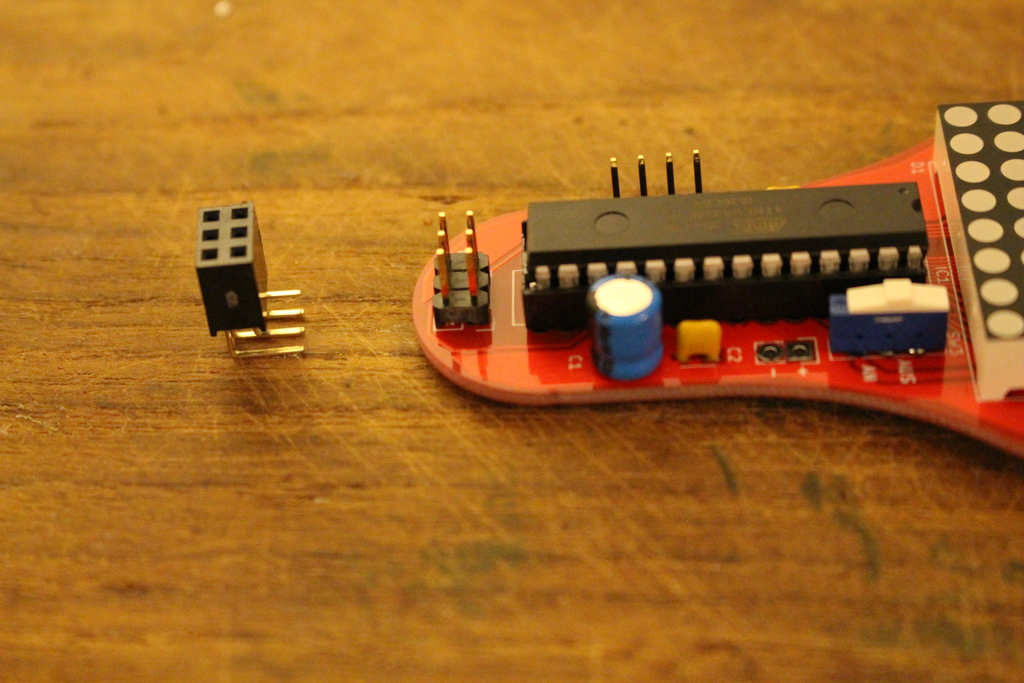
\includegraphics[width=\textwidth]{Bilder2019/IMG_6482.JPG}
	%\captionof{figure}{}
	%\label{fig:}
\end{minipage}
\begin{minipage}[b]{0.5\textwidth}
	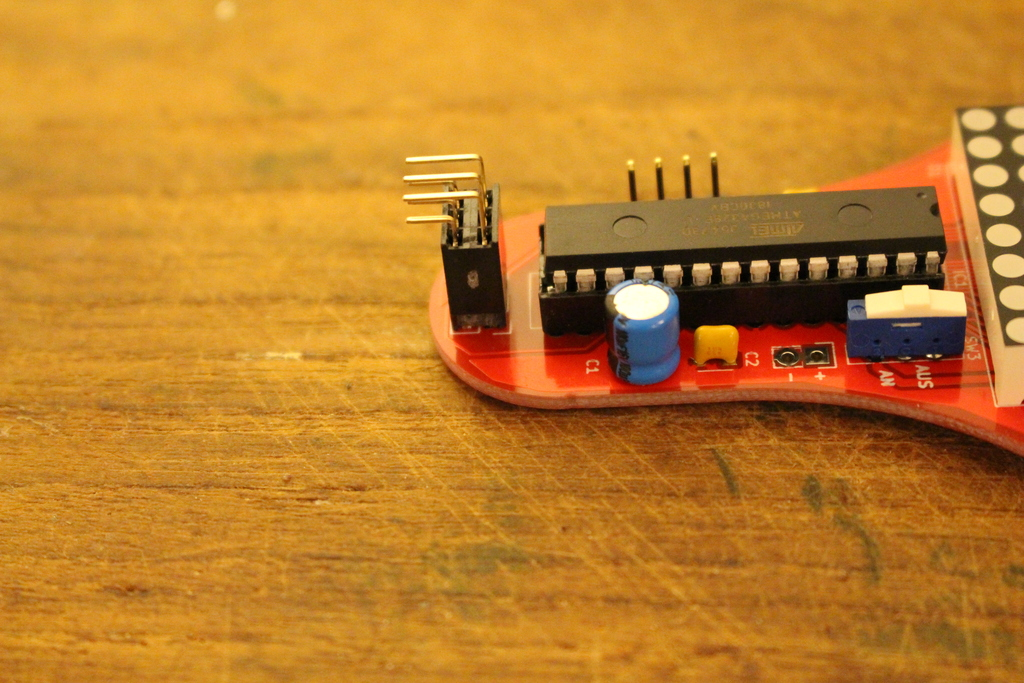
\includegraphics[width=\textwidth]{Bilder2019/IMG_6483.JPG}
	%\captionof{figure}{}
	%\label{fig:}
\end{minipage}

\vspace{0.5cm}

\begin{minipage}[b]{0.5\textwidth}
	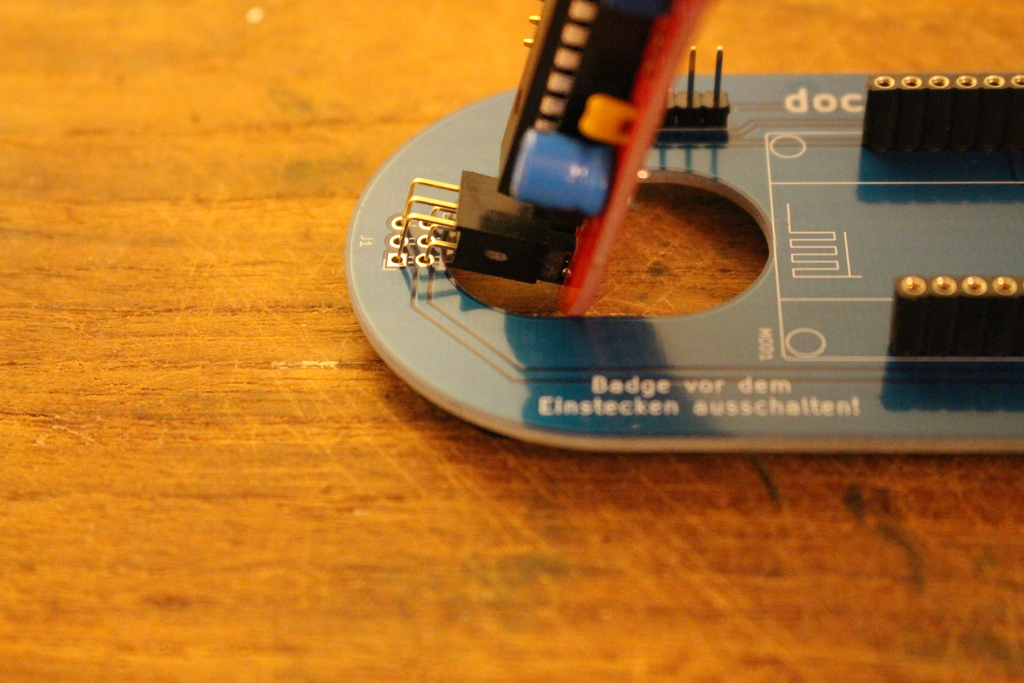
\includegraphics[width=\textwidth]{Bilder2019/IMG_6484.JPG}
	%\captionof{figure}{}
	%\label{fig:}
\end{minipage}
\begin{minipage}[b]{0.5\textwidth}
	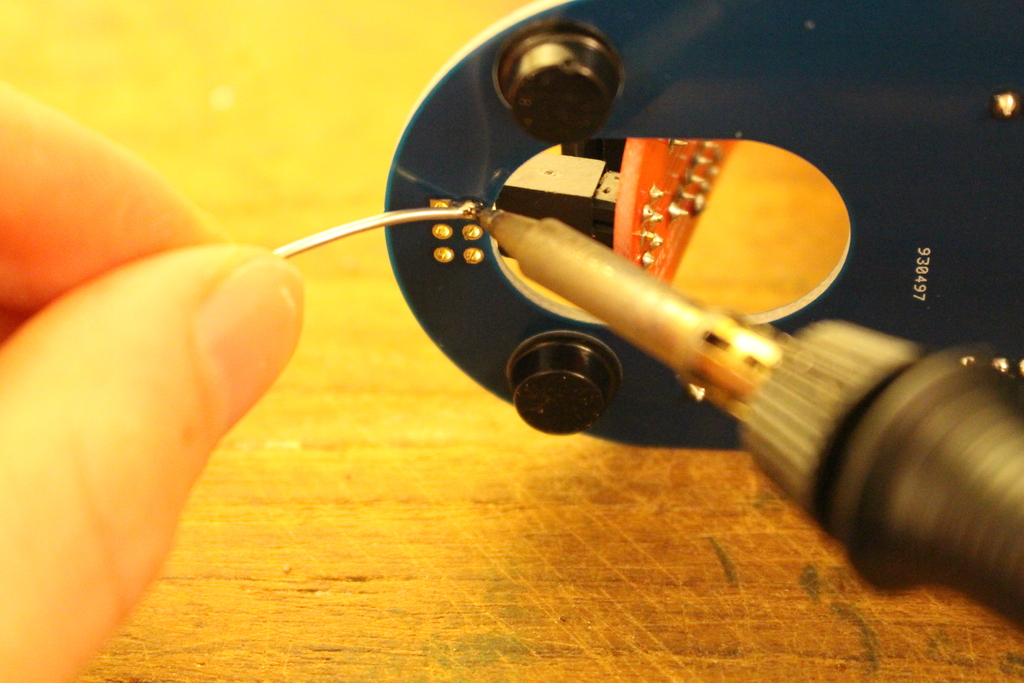
\includegraphics[width=\textwidth]{Bilder2019/IMG_6485.JPG}
	%\captionof{figure}{}
	%\label{fig:}
\end{minipage}

\vspace{0.5cm}

\begin{minipage}[b]{0.5\textwidth}
	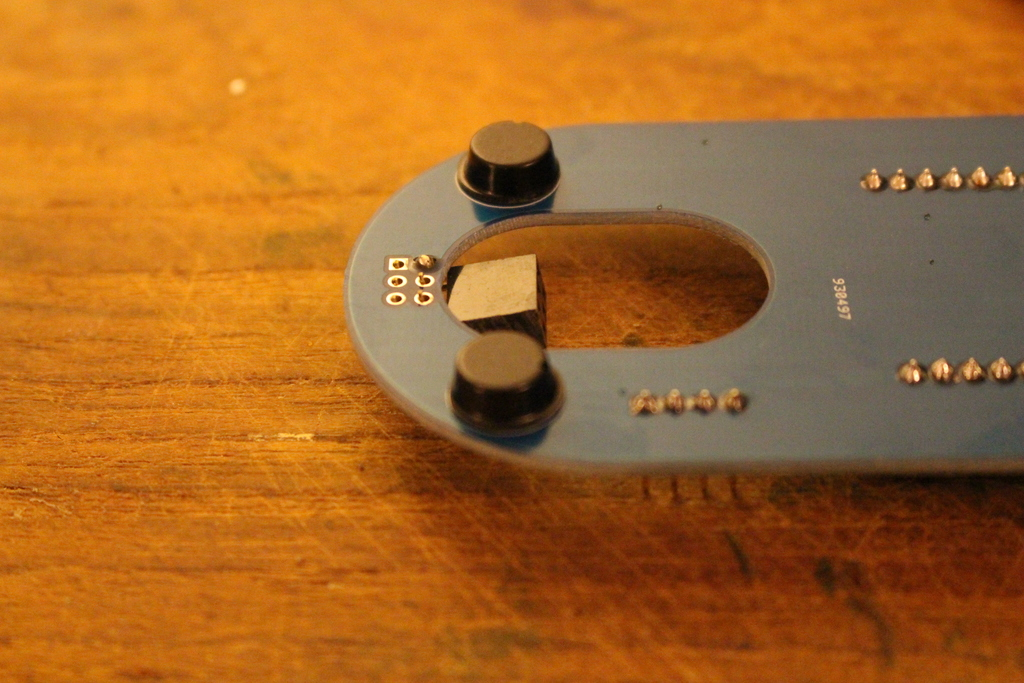
\includegraphics[width=\textwidth]{Bilder2019/IMG_6486.JPG}
	%\captionof{figure}{}
	%\label{fig:}
\end{minipage}
\begin{minipage}[b]{0.5\textwidth}
	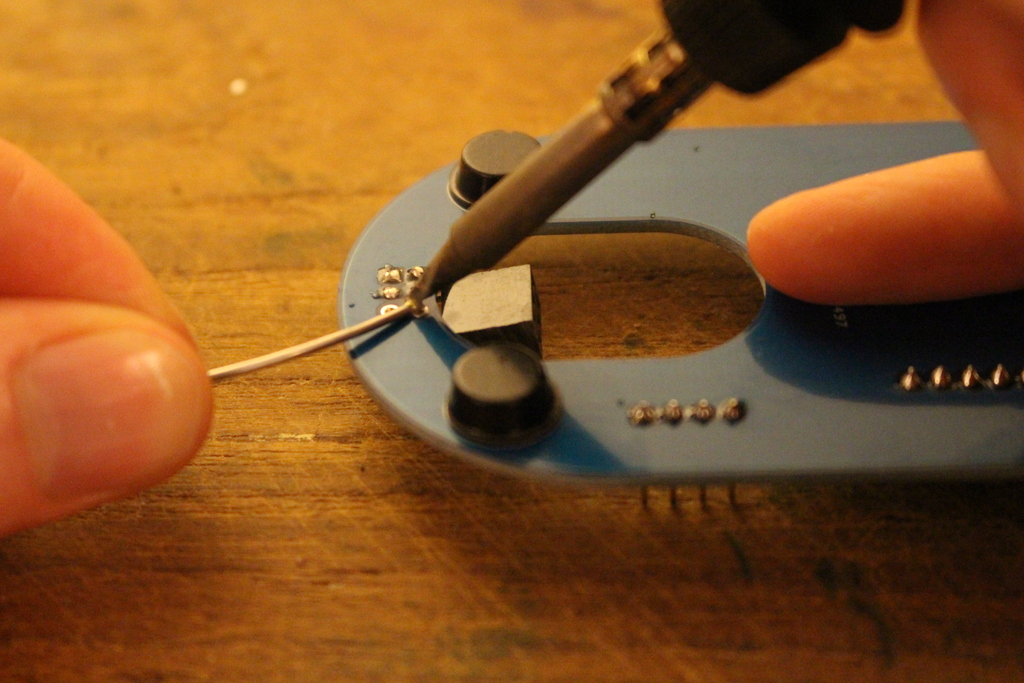
\includegraphics[width=\textwidth]{Bilder2019/IMG_6487.JPG}
	%\captionof{figure}{}
	%\label{fig:}
\end{minipage}

\vspace{0.5cm}

\begin{minipage}[b]{0.5\textwidth}
	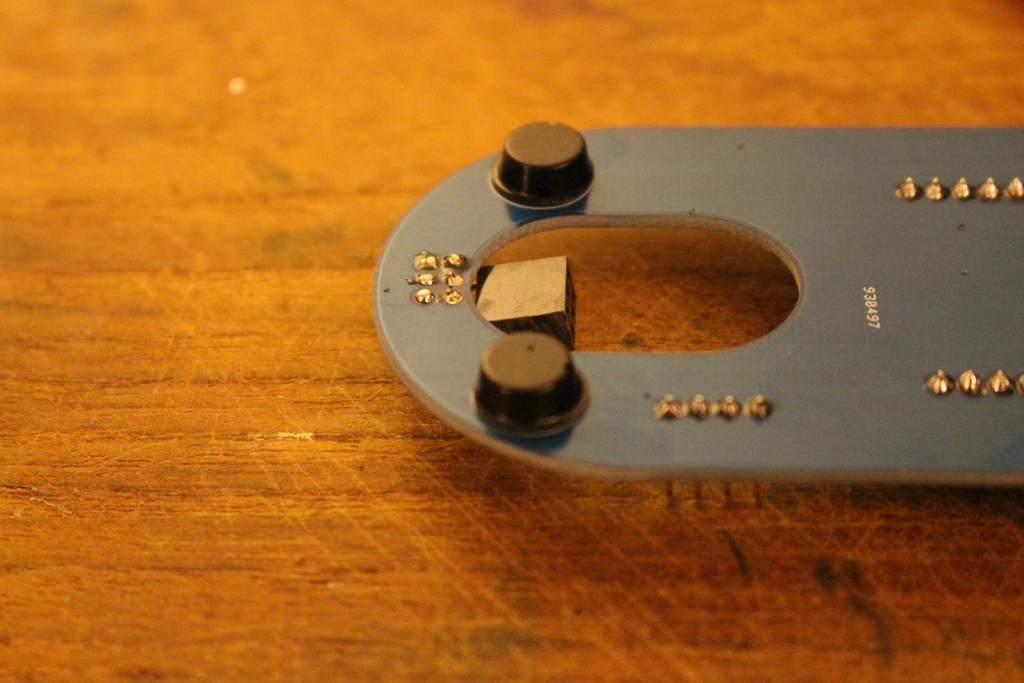
\includegraphics[width=\textwidth]{Bilder2019/IMG_6488.JPG}
	%\captionof{figure}{}
	%\label{fig:}
\end{minipage}
\begin{minipage}[b]{0.5\textwidth}
	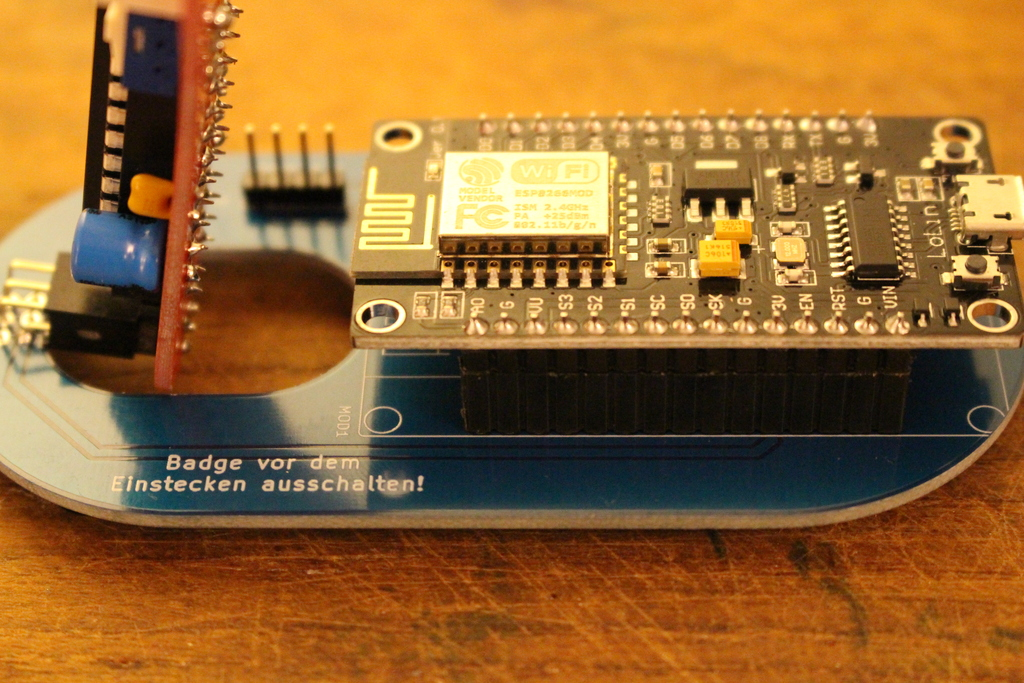
\includegraphics[width=\textwidth]{Bilder2019/IMG_6489.JPG}
	%\captionof{figure}{}
	%\label{fig:}
\end{minipage}

\subsection{Jumperkabel}

Nun musst du mit dem Jumperkabel noch das Dock mit dem Macherdaach-Badge verbinden. Dazu steckst du das eine Ende des Jumperkabels an den Pin am Dock, der mit einem von der Platine wegzeigenden Pfeil beschriftet ist und das andere Ende an den Pin am MacherdaachBadge, der mit einem in die Platine hineinzeigenden Pfeil beschriftet ist.

\vspace{1cm}

\begin{minipage}[b]{0.5\textwidth}
	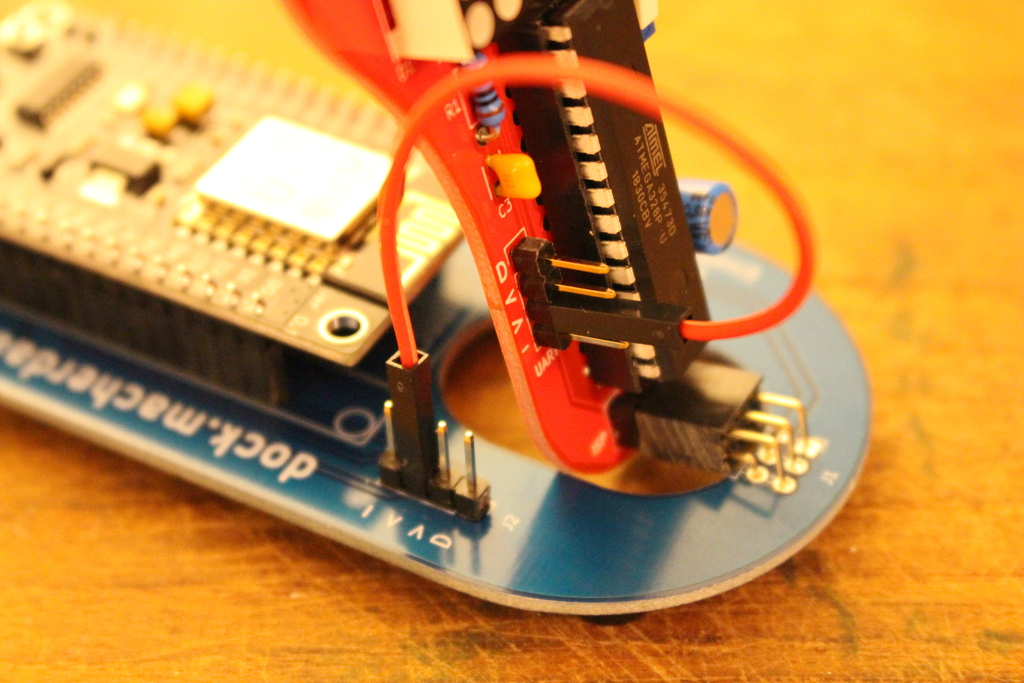
\includegraphics[width=\textwidth]{Bilder2019/IMG_6490.JPG}
	%\captionof{figure}{}
	%\label{fig:}
\end{minipage}

\subsection{Programmieren}

Bitte lies diese Anleitung zu Ende und erfahre, wie du dein Dock konfigurieren kannst, bevor du es an der Programmierstation programmieren lässt.

\subsection{Konfiguration}

Du hast dich sicherlich gefragt, wozu das Dock überhaupt gut ist und was es denn eigentlich tut.\\

Das ist eigentlich ganz einfach. Wenn dein Dock noch nie konfiguriert wurde (so wie jetzt) und du es mit Hilfe eines Handyladegräts mit Spannung versorgst, öffnet es einen WLAN-Hotspot. Du kannst dich dann mit deinem Smartphone mit diesem Hotspot verbinden und die Konfiguration vornehmen.

Dazu öffnest du den Browser, tippst auf WiFi Konfigurieren, wählst ein WLAN aus und gibst das zugehörige Passwort ein.
Hier auf dem Macherdaach kannst du "`Neuland"' benutzen mit dem Passwort "`12345678"'.

Immer wenn sich das Dock mit dem konfigurierten Passwort verbinden kann, wird es das tun und die aktuelle Uhrzeit aus dem Internet abfragen und als Laufschrift auf dem Badge anzeigen.

Wenn das Dock sich mit dem konfigurierten WLAN nicht verbinden kann, öffnet es wie zu Beginn einen WLAN-Hotspot, sodass du ein neues WLAN konfigurieren kannst.

\vspace{1cm}

\begin{minipage}[b]{0.5\textwidth}
	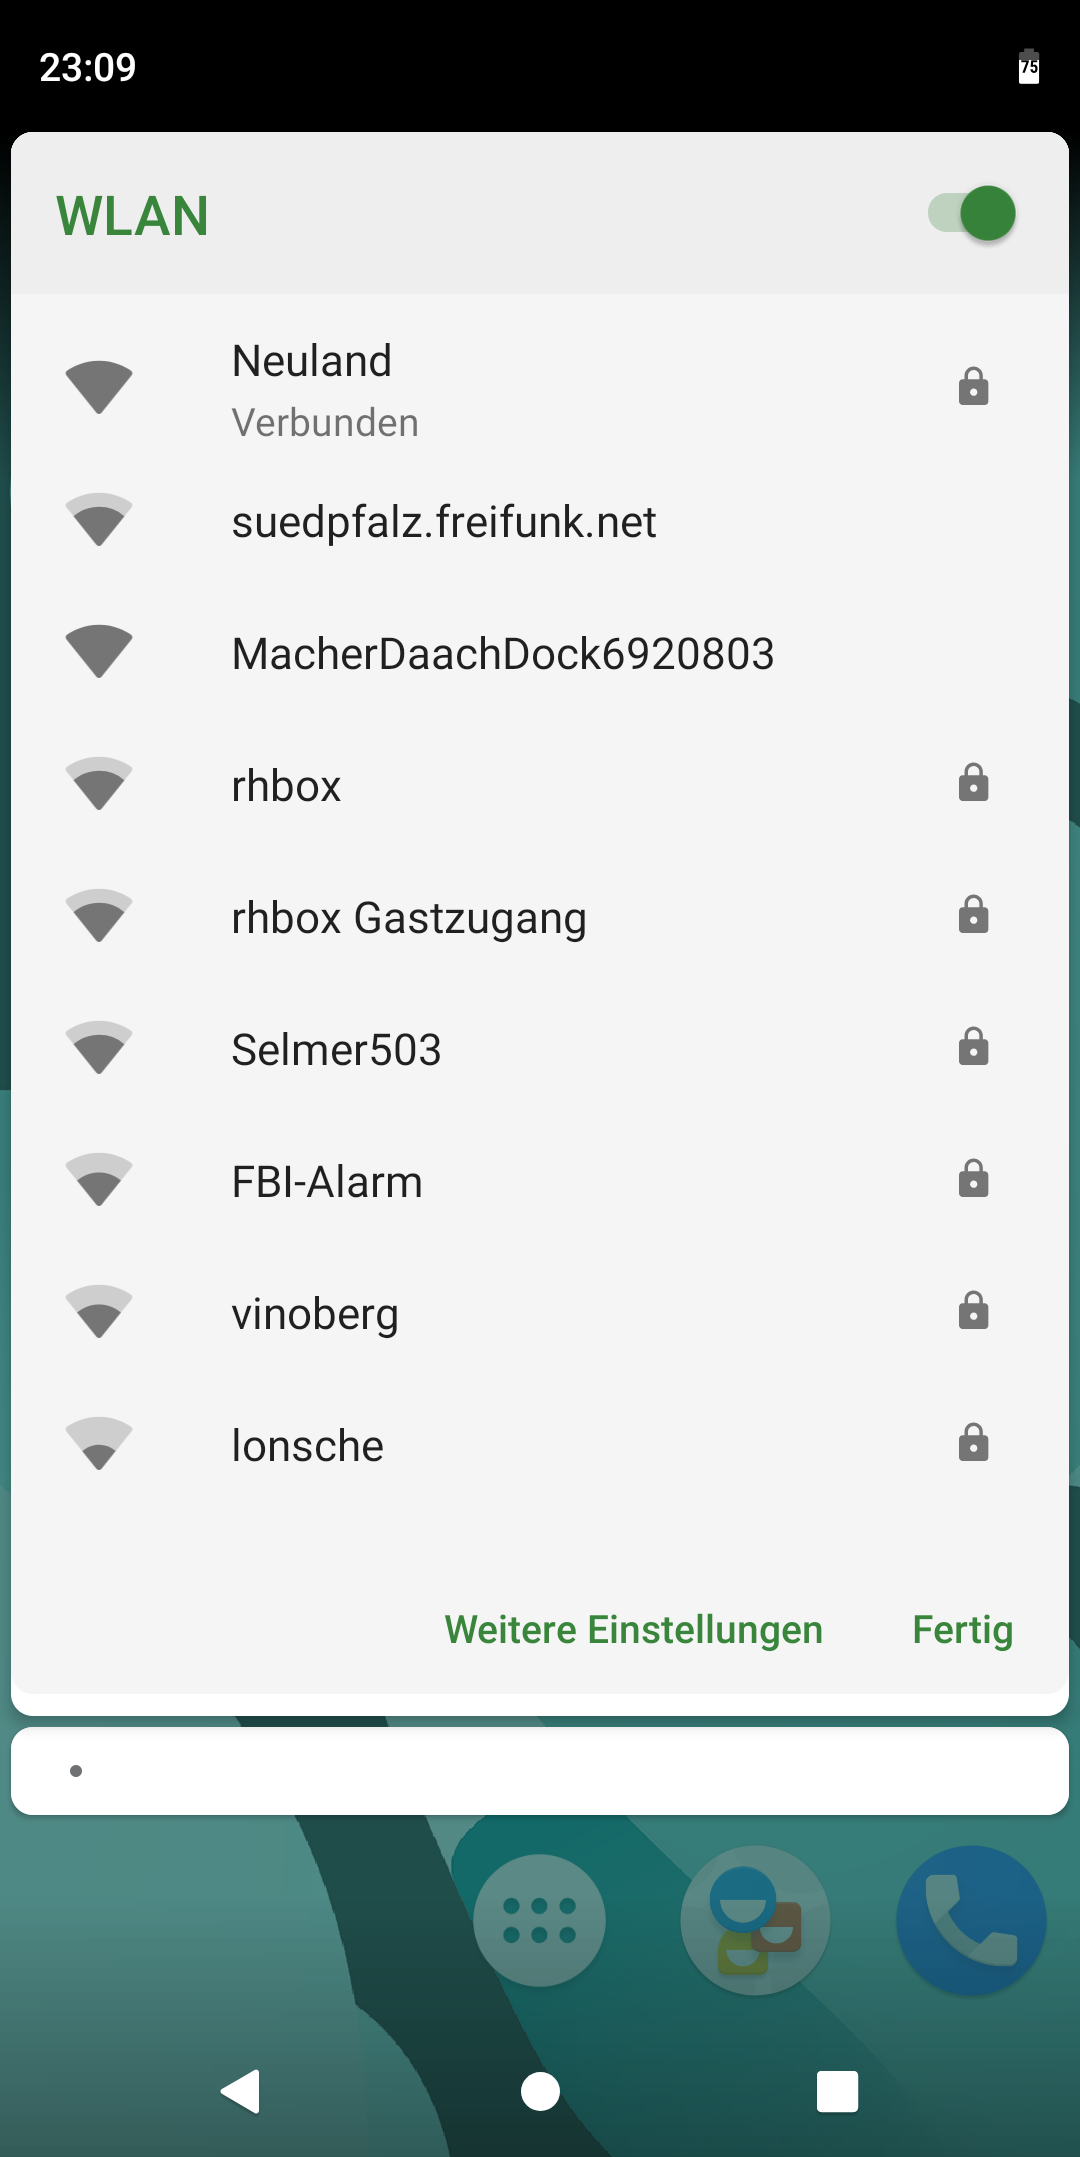
\includegraphics[width=\textwidth]{Bilder2019/Screenshot_20190918-230918_Nova_Launcher.png}
	%\captionof{figure}{}
	%\label{fig:}
\end{minipage}
\begin{minipage}[b]{0.5\textwidth}
	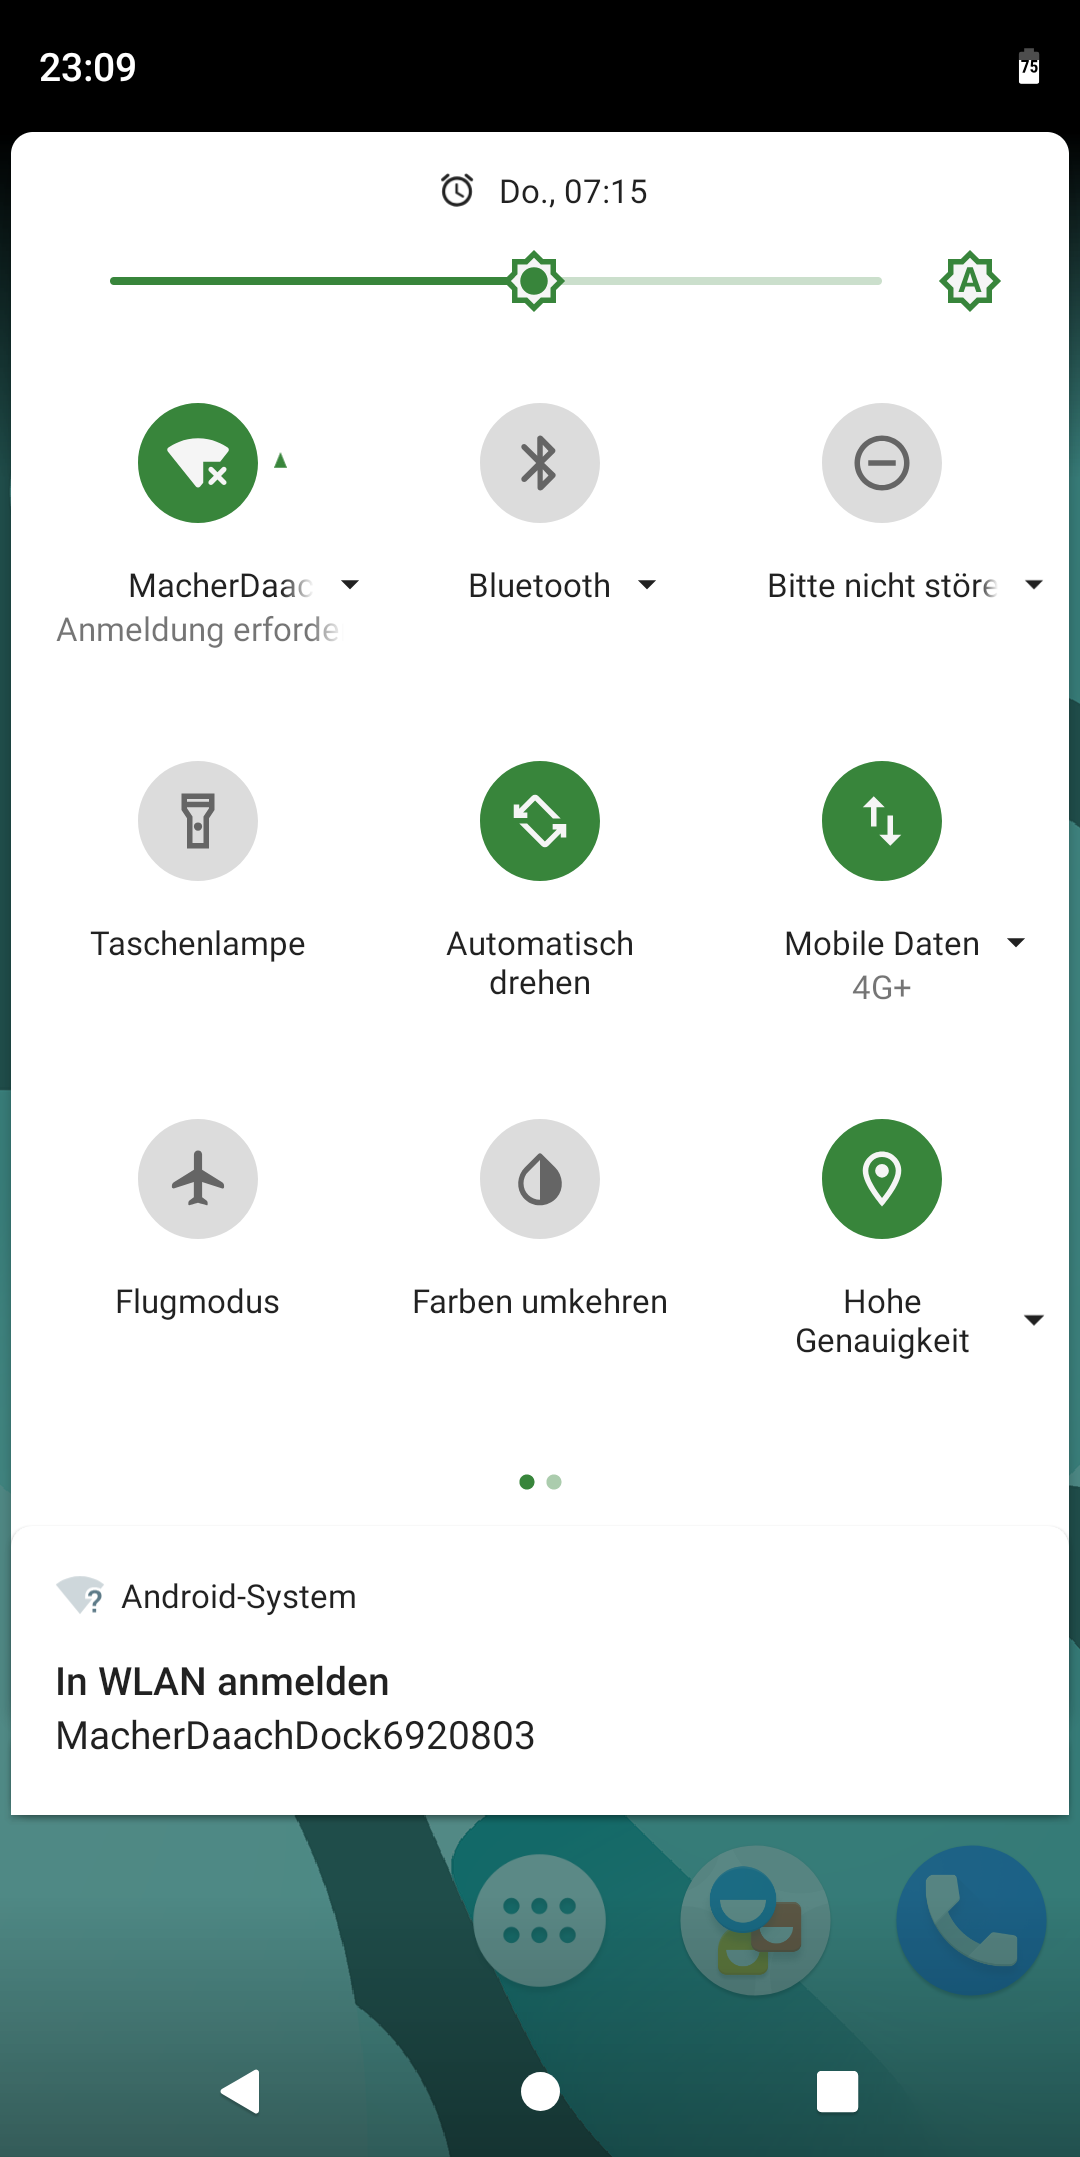
\includegraphics[width=\textwidth]{Bilder2019/Screenshot_20190918-230930_Nova_Launcher.png}
	%\captionof{figure}{}
	%\label{fig:}
\end{minipage}

\vspace{0.5cm}

\begin{minipage}[b]{0.5\textwidth}
	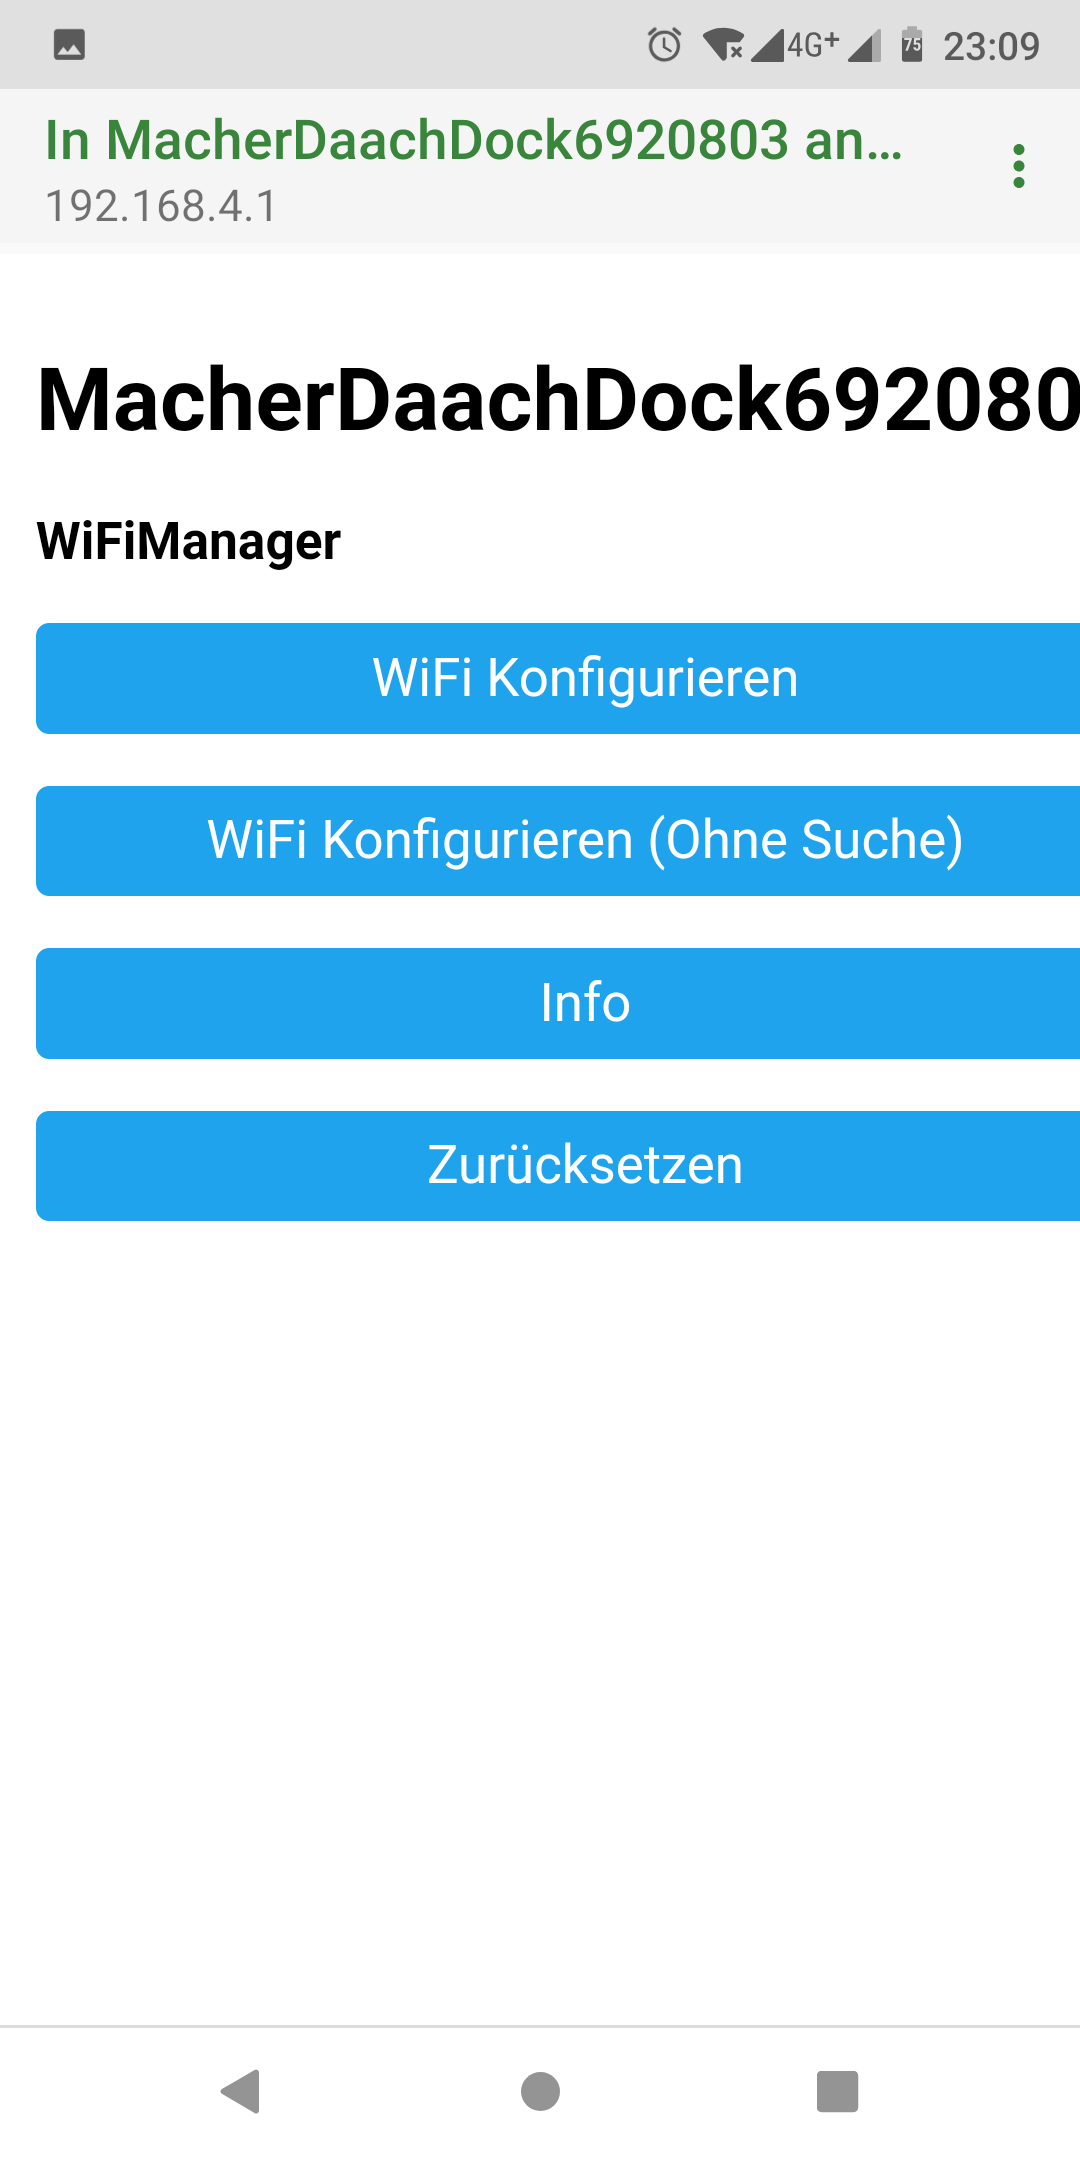
\includegraphics[width=\textwidth]{Bilder2019/Screenshot_20190918-230936_CaptivePortalLogin.png}
	%\captionof{figure}{}
	%\label{fig:}
\end{minipage}
\begin{minipage}[b]{0.5\textwidth}
	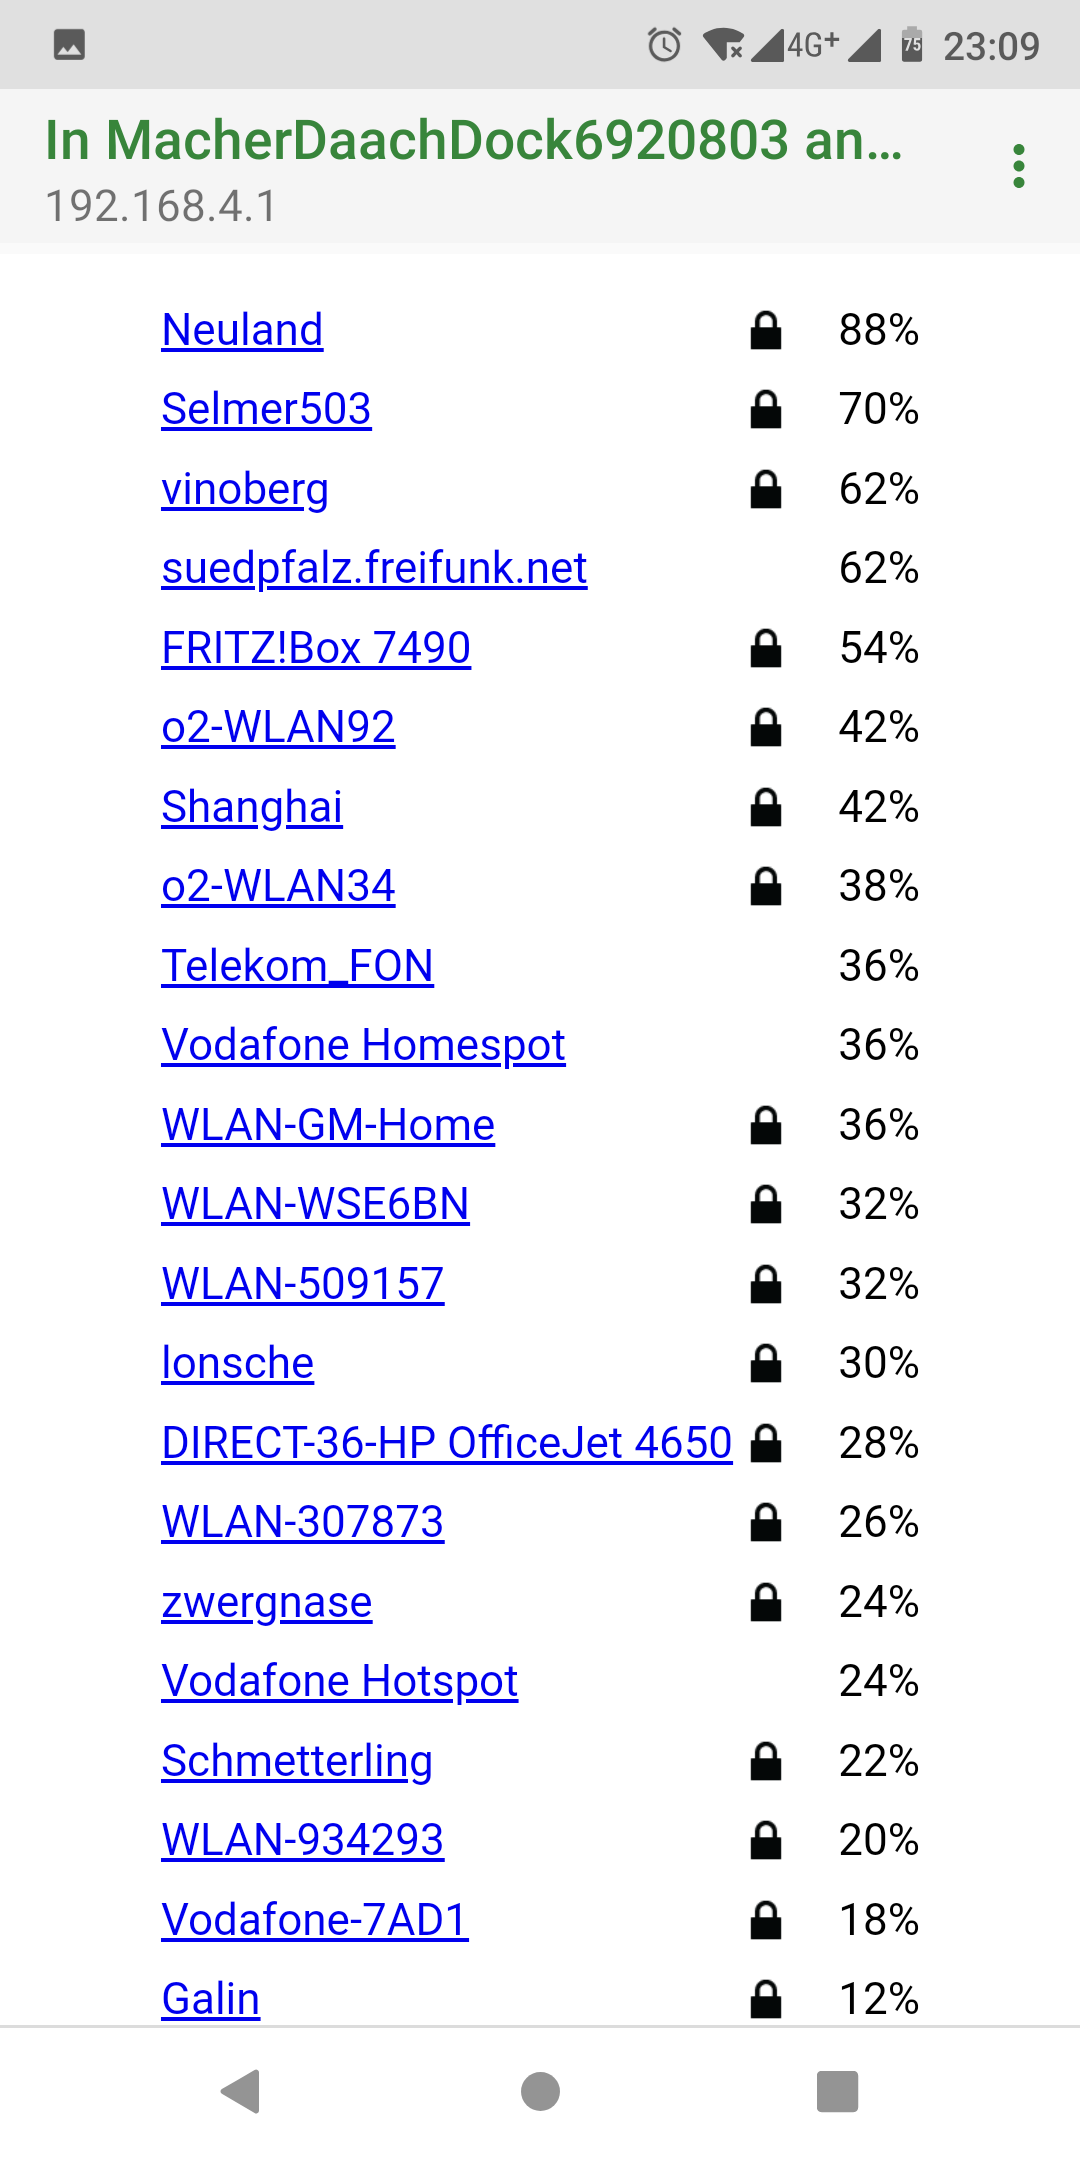
\includegraphics[width=\textwidth]{Bilder2019/Screenshot_20190918-230951_CaptivePortalLogin.png}
	%\captionof{figure}{}
	%\label{fig:}
\end{minipage}


\vspace{0.5cm}

\begin{minipage}[b]{0.5\textwidth}
	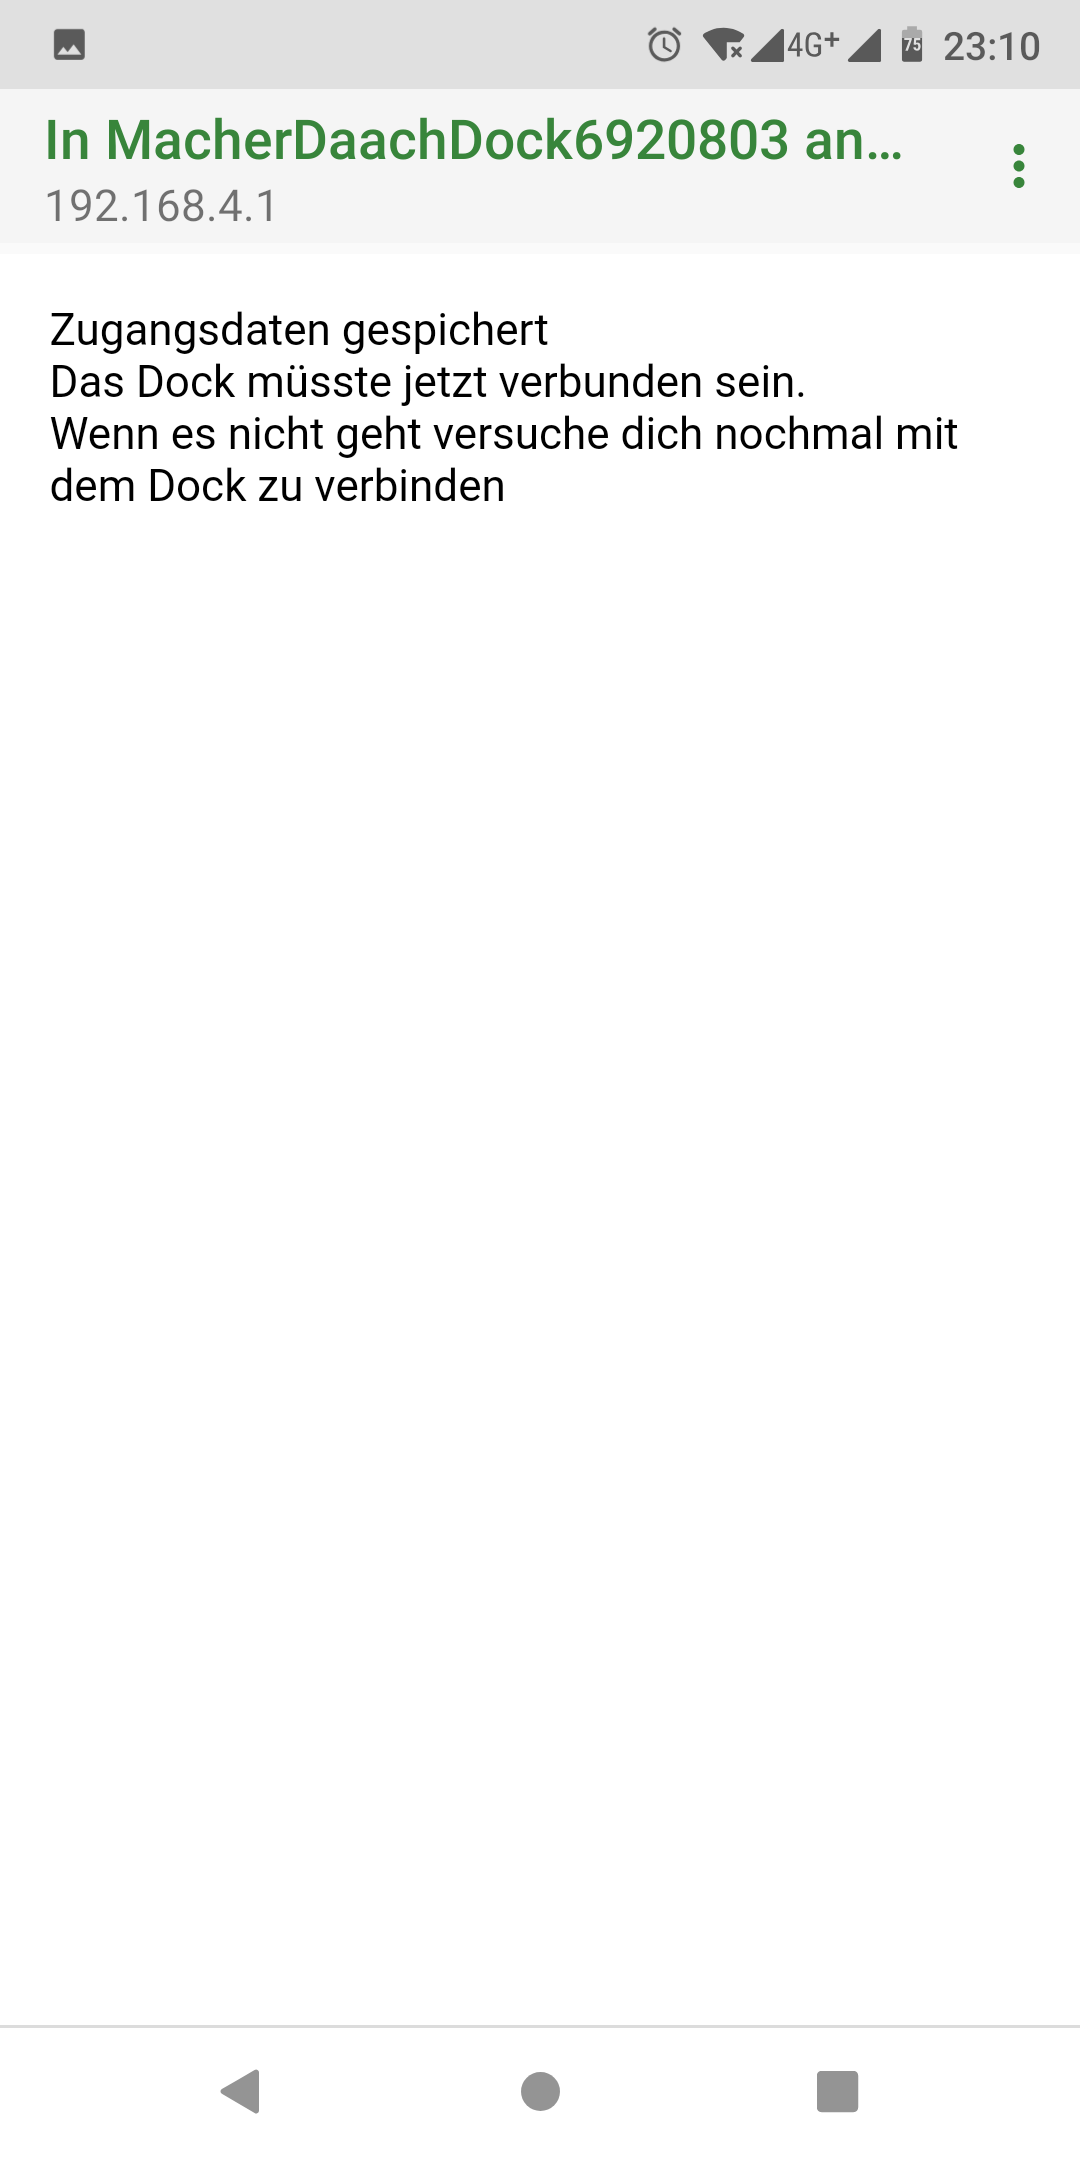
\includegraphics[width=\textwidth]{Bilder2019/Screenshot_20190918-231047_CaptivePortalLogin.png}
	%\captionof{figure}{}
	%\label{fig:}
\end{minipage}

\subsection{Test}

Um zu testen, ob die Uhrzeit richtig bei dir angezeigt wird, kannst du dich an eines der Micro-USB-Kabel anschließen und dein WLAN konfigurieren.\\

Bitte beachte stehts, dass MacherdaachBadge auszuschalten, wenn du es mit dem Dock verbindest, sonst ist die Batterie ruck-zuck leer.\\

Zu Hause kannst du dann einfach ein altes Handy-Ladegeräte verwenden um deine super coole Macherdaach-Badge-Uhr mit der nötigen Spannung zu versorgen.\\

Wir wünschen super viel Spaß damit.

\bibliographystyle{plain}
\bibliography{references}
\end{document}
